\documentclass[a4paper,12pt]{extreport}
\usepackage{fontspec}
\setmainfont{Times New Roman}

\usepackage{float}
\usepackage[russian,english]{babel}
\usepackage{csquotes}
\usepackage{amsmath}
\usepackage{amsthm}
\usepackage{amssymb}
\usepackage{ragged2e}
\usepackage[left=30mm, right=10mm, top=20mm, bottom=20mm]{geometry}

\usepackage{graphicx} 
\graphicspath{{figures/}}
\usepackage{ragged2e}
\usepackage{microtype}
\usepackage{titlesec}

\usepackage[hidelinks]{hyperref}

\usepackage{blindtext}
\usepackage{listings}
\usepackage{xcolor}

\lstdefinestyle{php}{
    language=PHP,
    basicstyle=\footnotesize\ttfamily,
    keywordstyle=\color{blue},
    stringstyle=\color{red},
    commentstyle=\color{green},
    morecomment=[l][\color{magenta}]{\#},
    tabsize=2,
    frame=single,
    breaklines=true,
    breakatwhitespace=true,
    postbreak=\mbox{\textcolor{red}{$\hookrightarrow$}\space},
    showstringspaces=false,
    numbers=left,
    numberstyle=\tiny\color{gray},
    captionpos=b,
    belowcaptionskip=1\baselineskip,
    xleftmargin=\parindent,
    columns=fullflexible,
    keepspaces=true,
    escapechar=|,
}

\usepackage[%
backend=biber
,bibstyle=apa
,citestyle=numeric-comp
,sorting=none
,sortcites=true
,block=none
]{biblatex}
\addbibresource{bibliography.bib}
\makeatletter
\RequireBibliographyStyle{numeric-comp}
\makeatother

\def\myauthor{Alexandr Ossipov, Daulet Lepessov, Nurlan Darzhanov, Saya Oryskhan}
\def\mycoach{Ramis Akhmedov, PhD}
\def\mytitle{The Application of SkillSwap}
\def\mydegree{Bachelor in Information Systems}
\def\mydegreecode{6B06101 } 

\begin{document}
    \begin{titlepage}
\begin{center}


\includegraphics[width=0.2\textwidth]{figures/Log_SDU.png}
\vspace{0.5cm}
\large 
\par
\textbf{SDU University} 

\large 
\textbf{Faculty of Engineering and Natural  Science}

\vspace{5cm}

\Large 

\textbf{\mytitle}

\par

\vspace{0.5cm}
\large
 Design and implementation of the university admission platform for high school graduates.
\begin{center}
\Large\textbf{Alexandr Ossipov} \\
\textbf{Daulet Lepessov} \\
\textbf{Nurlan Darzhanov} \\
\textbf{Saya Oryskhan}
\end{center}

\vspace{2cm}
\large
\mydegreecode - “Information Systems”

\vfill
\large
Kaskelen, 2024 \centering

\end{center}
\end{titlepage}
    \newpage
\pagestyle{empty}
\begin{center}


\includegraphics[width=0.2\textwidth]{figures/Log_SDU.png}

\includegraphics[width=0.23\textwidth]{figures/Faculty.png}
\vspace{0.5cm}
\Large 
\par
\textbf{SDU University} 

\Large \textbf{Faculty of Engineering and Natural  Science}

\vspace{2cm}
\normalsize\hspace{9.5cm} Dean of Faculty \\
\normalsize\hspace{9.5cm} Assis. Prof., PhD Ramis A. \\
\normalsize\hspace{9.5cm}\underline{\hspace{6cm}} \\
\normalsize\hspace{9.5cm}«\underline{\hspace{0.5cm}}»\underline{\hspace{4cm}}2024y. \\

\vspace{2cm}
\Large
\textbf{\mytitle}
\par
\vspace{0.5cm}
 \normalsize Design and implementation of the university admission platform for high school graduates.\\
    \vspace{0.5cm}
    \mydegreecode - ``Information Systems''\\
    \normalsize
    \vspace{1cm} 
    \textbf{Supervisor:}\raggedleft \hspace{5cm} Ramis A.\\
    \vspace{0.5cm}
    \textbf{Student:}\raggedleft \hspace{4.5cm} Alexandr O.\\
    \vspace{0.5cm}
    \textbf{Student:}\raggedleft \hspace{5cm} Daulet L.\\ 
    \vspace{0.5cm}
    \textbf{Student:}\raggedleft \hspace{4.9cm} Nurlan D.\\ 
    \vspace{0.5cm}
    \textbf{Student:}\raggedleft \hspace{5.3cm} Saya O.\\ 

\vfill
Kaskelen, 2024 \centering
\end{center}

    \newpage
\pagestyle{plain}

\begin{center}
    \Large
    \textbf{Abstract}
\end{center}
Today, information technology is developing steadily and plays an important role in improving various areas, including education. To ensure ease and convenience, innovative solutions and ideas are emerging in each area, which improve processes on a daily basis. In this context, through mutually beneficial exchange of skills and finding financing for start-up projects, they do not stand still and actively use digitalization based on information technology. SkillSwap - the mission of our application and website is to make it easier for students to gain new knowledge and put it into practice and gain new skills that they will expect, as well as an important skill is a way of communication for our students that they will need throughout their lives, and integrate a crowdfunding platform where students can share their project and get donations on that. This project aims to be informative and interesting, as well as to have the opportunity to be integrated into an information system based on schools and universities.
    \newpage
\pagestyle{plain}

{\selectlanguage{russian}
\begin{center}
    \Large
    \textbf{Аңдатпа}
\end{center}
\hspace*{0.5cm} Бүгінгі, таңда Ақпараттық технологиялар үнемі дамып келеді және білім беруді қоса алғанда, әртүрлі салаларды жетілдіруде маңызды рөл атқарады. Қарапайымдылық пен ыңғайлылықты қамтамасыз ету үшін әр салада процесті күнделікті жетілдіретін инновациялық шешімдер мен идеялар пайда болады. Бұл тұрғыда өзара тиімді дағдылармен алмасу және стартап-жобаларды қаржыландыру арқылы олар бір орында тұрмайды және ақпараттық технологияларға негізделген цифрландыруды белсенді пайдаланады. SkillSwap - біздің қосымшамыз бен веб-сайтымыздың миссиясы бұл студенттерге жаңа білім алуды және оларды іс жүзінде қолдануды жеңілдету, сонымен қатар жаңа дағдыларды игеру олар таңдаған, сондай - ақ маңызды дағды-бұл біздің студенттер үшін қарым-қатынас тәсілі олар өмір бойы қажет және студенттер өз жобаларымен бөлісе алатын краудфандинг платформасын біріктіру және бұл үшін қайырымдылық алыңыз. Бұл жоба ақпараттық және қызықты болуы керек, сонымен қатар мектептер мен университеттерге негізделген ақпараттық жүйеге интеграциялануы керек.
}
    \newpage
\pagestyle{plain}

{\selectlanguage{russian}
\begin{center}
    \Large
    \textbf{Аннотация}
\end{center}
\hspace*{1cm} Сегодня, информационные технологии неуклонно развиваются и играют важную роль в усовершенствовании различных областей, включая образование. Для обеспечения простоты и удобства в каждой области появляются инновационные решения и идеи, ежедневно совершенствующие процесс. В этом контексте, благодаря взаимовыгодному обмену навыками и финансированию стартап-проектов, они не стоят на месте и активно используют цифровизацию, основанную на информационных технологиях. SkillSwap - миссия нашего приложения и веб-сайта это облегчить  студентам получение новых знаний и применение их на практике, а также приобретение новых навыков которые они предпочтут, а также важный навык - это способ коммуникации, для наших студентов которые им понадобиться на протяжении всей жизни, и интегрировать краудфандинговую платформу, где студенты могут поделиться своим проектом и получать пожертвования на это. Этот проект должен быть информативным и интересным, а также иметь возможность быть интегрированным в информационную систему на базе школ и университетов.
}
    \tableofcontents
    
    \chapter{Introduction}\label{ch:intro}

\section{Motivation}\label{motivation}
\hspace*{0.5cm} Today, after the Covid - 19 pandemic \cite{covid}, information technology is moving at an incredible speed within Kazakhstan and around the world, many online learning platforms are being created where users learn new skills and apply them in practice. Our SkillSwap \cite{skillswap} project aims to unite students into one community where they can exchange skills, ask questions, and answer them, it is a mutually beneficial exchange of skills, and a student can also receive funding for his project if he really innovates, if the investor himself sees it.The platform itself allows you to find other students who are also interested in learning something new, and a paid exchange is also possible, depending on the purpose of the students. The motivation and mission of our project itself come from effective learning, proper planning, and application of new knowledge in practice (depends on the motivation and vision of the students themselves); our platform is the place (together) where students can find and learn something new, answers to questions within the platform, that is, each student can ask a question and answer it and also give a rating to the question, that is, is the question good or not, all students should know how to ask a question to learn this -  nometa.xyz \cite{nometa} encouraging students to correctly use communication skills that will be useful to them in the future. Today there is such a problem that students are afraid to communicate, to make new acquaintances. There is a risk that a student after graduation will not find friends and connections and will grieve about this. In the next chapters, we will consider this problem in more detail.

\newpage
\section{Aims and Objectives}\label{aimsobj}
\justifying
\hspace*{0.5cm} Our project objective is to create a platform for students to mutually benefit from the exchange of skills in order to learn something new and find new connections within the people and university, as well as being able to ask any question on the platform and answer others, and implement a crowdfunding platform \cite{crowdfunding} for devouring any project. Taking this into account, we next identified \nameref{aimsobj}.

\par
\flushleft
\textbf{Aims:}
\begin{itemize}
\justifying
  \item Creating a platform within the university aimed at exchanging skills between students in order to improve their communication skills and technique skills.
  \item Increasing students ability to use the platform to share knowledge and experiences, giving them the opportunity to ask questions, answer them and evaluate their usefulness, similar to popular resources like Stack Overflow \cite{stackoverlow} and headhunter.kz \cite{headhunter} or reddit.com \cite{reddit}.
  \item Support student’s projects on the platform by providing them with tools to finance them and implement their ideas, including using a donation system that allows investors to support promising projects.
\end{itemize}

\textbf{Objectives:}
\begin{itemize}
\justifying
  \item The development of a website (describes in \nameref{back} part) platform and an application \nameref{ios} that makes it possible to register on the platform, which makes it possible to use 100 percent of the platform's functionality and also create their profiles.
  \item The development of a kind of mechanism for the exchange of skills, and this is a chat so that users can communicate, also ask questions and give answers to them, and also rate the question whether it is correctly asked or not.
  \item Creating a crowdfunding \cite{crowdfunding} section for the exhibition of personal projects from students who need financing for future investors.
  \item Creating a simple and proper interface for users to use the application better.
  \item Implement security for users of SHA-256 data encryption and personal chat history information.  
\end{itemize}

\newpage
\section{Problem statement}\label{prblstatm}
\begin{figure}[ht]\label{fig:sstats}
  \centering
  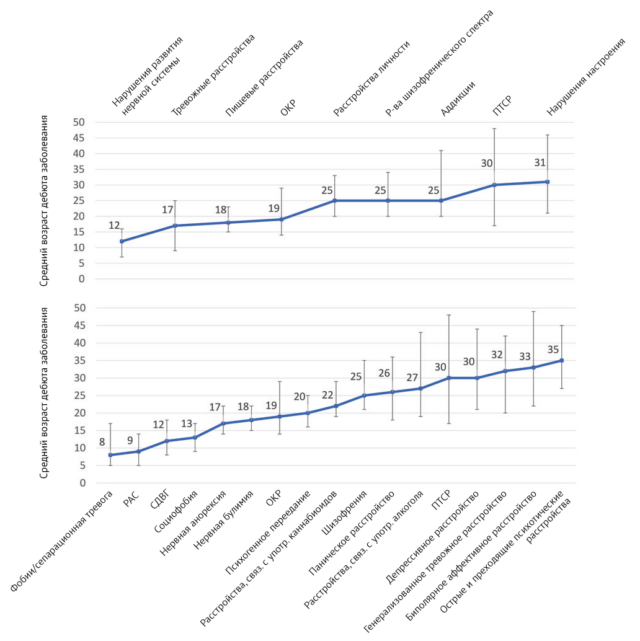
\includegraphics[width=0.8\linewidth]{figures/Students_issue.png}
  \caption{A statistics about students age and their issues.}
\end{figure}

\vspace{0.5cm}
\justifying
 Today, most students face a lack of opportunities and fear in communication, as well as to ask for help for mutually beneficial exchange of skills and also experience and support for their educational projects and ideas within the universities themselves. Despite the different online platforms on the internet and the initiatives of educational institutions, you say that universities have many clubs for the development of new abilities, for example: a music club or a programming club, yes, it helps but not everyone, perhaps the university gives a direction to help the student community, but it is not always not everyone uses it because of fear in communication. 
\par
\vspace{0.5cm}
Many of them have difficulties and fears in finding suitable resources and platforms and are also limited in communicating with students to get the necessary help to implement their ideas and projects or mutually beneficial exchange.  
\newpage
Limited access (not in all universities) to high-quality educational materials, some materials may be outdated, restrictions on social contact, some students are afraid to make contact, which may affect in the future and lack of financial support for their ideas, implementation, influence, and so on, hinders the process of skill development, which may hinder the expansion of students' knowledge bases and the formation of professional relations within the university environment. 
\par
\vspace{0.5cm}
Such problems can affect the motivation of students, the realization of learning, personal development, and prospects for professional growth of students, which potentially affects both academic success and future careers.
Let's give some student fears, student fears are provocateurs of mental disorders in students.
As you can see in the picture above "\nameref{fig:sstats}", the main part of the students are young people \textbf{aged 17-25 years.} During this age period, the risk of many mental disorders increases. 
In 2021, the journal Molecular Psychiatry \cite{student-fears} published the results of a meta-analysis of 192 epidemiological studies from around the world, according to which the following psychopathologies are highly likely to debut at this age.

\par
\vspace{0.5cm}
\textbf{Eating disorders} - anorexia nervosa, bulimia nervosa, psychogenic overeating \cite{student-fears}.

\par
\vspace{0.5cm}
\textbf{Obsessive} compulsive disorders — are the appearance of obsessive, disturbing, or frightening thoughts (obsessions) and obsessive actions (compulsions) \cite{student-fears}.

\par
\vspace{0.5cm}
\textbf{Personality disorders}  —  are a distorted perception of reality and inadequate ways of responding to events \cite{student-fears}.

\par
\vspace{0.5cm}
\textbf{Schizophrenic disorders} — are fundamental disorders of thinking and perception that can be accompanied by auditory hallucinations, false memories, fantastic delusions, and social dysfunction \cite{student-fears}.

\par
\vspace{0.5cm}
\textbf{Addiction} — is the desire to escape reality and change your mental state with the help of psychotropic substances \cite{student-fears}.

\vspace{0.5cm}
Also, according to our survey, "\nameref{survqa6}" conducted in 2024 this semester, it turned out that when asked do you have a lot of friends at the university, it turned out that \textbf{53.8} percent have very few friends at universities, that is, they have few connections to live life in the future, that is, theoretically it will not be much harder to live who did not live who has more connections, therefore our application partially solves this problem.

\newpage
\section{Thesis Outline}\label{thesis}
\hspace*{0.5cm} The first chapter of our document is an "\nameref{ch:intro}" in which we describe our goals and motivation and describe the existing problem related to this project. The second chapter contains, "\nameref{ch:A}" information that will help readers understand how a mutually beneficial skills exchange project is carried out and not only help our country specifically for students in comparing other cases from different countries. In the third chapter, we describe the "\nameref{ch:B}" we used during the development of our project and how we distributed the responsibilities. In the fourth chapter, we describe about "\nameref{ch:C}" we do analyze competitive and product analysis by the topic our project. In the fifth chapter, we describe the "\nameref{ch:D}" of which stack technologies how we used starting our project from prototyping and ending MVP product and in the last section we describe the "\nameref{ch:E}" of the project and its further development.

    \chapter{Background}\label{ch:A}
\section{Literature review} \label{litrev}

\hspace*{1cm} In our world of non-stop informational flow and worldwide internet access, we have the means to access a vast array of information. Yet, students often encounter difficulties in various courses. In the articles "Massive Open Online Courses (MOOCs) \cite{massiveopenonlinecourses}: A Primer for University and College Board Members" and "SWATShare \cite{swatShare}– A web platform for collaborative research and education through online sharing, simulation, and visualization of SWAT models," we were introduced to projects aimed at assisting individuals with educational goals. 
\par
\vspace{0.5cm}
The most inspiring aspect of the first article \cite{massiveopenonlinecourses} was the project's similarity to on-campus courses, delivered synchronously on a defined schedule—usually on a weekly calendar basis—and offered for free. This prompted us to consider embedding similar features in our platform. We envisioned a platform where every student could share their skills, with options for free access, payment, or exchange for other skills or courses offered by fellow students. This approach would provide a more personalized learning experience, similar to receiving guidance from peers who have experienced similar challenges, thereby enhancing the effectiveness of education.
\par
\vspace{0.5cm}
In the second article \cite{swatShare}, we found it intriguing that the project emphasized the importance of collaboration among researchers and educators. This aligns with our main goal of facilitating easier, more interesting, and more useful communication among students for their educational benefit.
\par
\vspace{0.5cm}
Since we are aiming to embed crowdfunding \cite{crowdfunding} functionality into our project, we found the article "Crowdfunding: Why People Are Motivated to Post and Fund Projects on Crowdfunding Platforms" quite informative. This article provided us with insights into how crowdfunding works from both the creator and funder perspectives. It highlighted how social interactions play a crucial role in creating a feeling of belonging to a community that shares common interests and values, especially among those who fund projects. Additionally, the article discussed the psychological aspects of crowdfunding, highlighting factors such as sympathy, empathy, guilt, happiness, and identity, which influence individuals' motivations for investing money into projects. It also addressed how the framing of a funding request can impact the donation amount and the potential limitations we might encounter in the process.

\newpage
\section{International and local cases analysis} \label{intandloc}

\hspace*{1cm} In the process of brainstorming our project's problem statement, we considered already existing projects created for students to develop a competitive project. We decided to examine six different cases for the three main functionalities of our app: skill sharing, Question Answer, and crowdfunding, with 1 local and 1 international existing solutions for each functionality.

\begin{enumerate}
    \item First, let’s consider skill sharing functionality in next platforms:

     \textit{SkillShare} is a platform designed for sharing skills, enabling users to either purchase or upload their courses. It is a globally recognized platform that inspired us, but we observed that despite feedback, many course-selling platforms like skillshare often lack effective communication and support. This led us to explore local application \textit{Olx}. Olx \cite{olx} features a service-sharing functionality that enhances user interaction significantly. However, its major drawback lies in the lack of security measures, resulting in numerous scams and a suspicious reputation. In response, we conceived the idea of launching a platform accessible only to authenticated users, exclusively students. Through thorough analysis, we identified the strengths of both platforms and endeavoured to address their shortcomings.

     \item Next, let’s consider Question Answer functionality in next platforms:

     Our team drew inspiration from the platform \textit{Stack Overflow} \cite{stackoverlow}, which has provided answers to our questions on numerous occasions. With its wide user base, responses to questions are swift, and the variety of people who contribute brings different viewpoints, which is a significant benefit. However, we identified a limitation: Stack Overflow \cite{stackoverlow} created exclusively for developers, whereas we aspire to create a platform where students from various fields can engage in discussions and seek solutions to their questions. In our quest for alternatives, we explored the Russian platform \textit{Znanija.com} \cite{znanija}, tailored for school students and covering a broader range of subjects. Nevertheless, a significant drawback became apparent: the platform's limited user base and language barrier, resulting in fewer responses to submitted questions and issues. Another common disadvantage in both of these platforms is also authentication, allowing any user to provide answers, consequently, there may be no way to follow up with the user who previously answered. Therefore, in our application, we aim to enable authenticated students to engage in discussions about topics of interest and establish connections with users who provide answers, similar to interactions on social media platforms.

  \item Finally, let’s consider crowdfunding functionality in next platforms:

We came across an interesting student-centered crowdfunding platform called \textit{StudentBackr}, which is designed to help students cover various fees and finance projects related to student life. However, we discovered that it operates exclusively in European countries.So we looked into local \textit{Start-time.kz} \cite{starttime} platform, which, although not specifically tailored for students, still allows investments in various areas of interest, which is excellent, but the platform's biggest flaw lies in its consistency. Platform is not actually user friendly and we could not get acquainted with terms and conditions or any policy. So we considered both strengths and weaknesses of these projects to develop competitive application. Our goal is to launch a user-centered crowdfunding platform that prioritizes usefulness and meets all requirements of such a significant project and will bring up projects with potential.
\end{enumerate}
    \chapter{Methodology}\label{ch:B}
\section{Agile}\label{agile}
\begin{figure}[ht]\label{fig:agile}
  \centering
  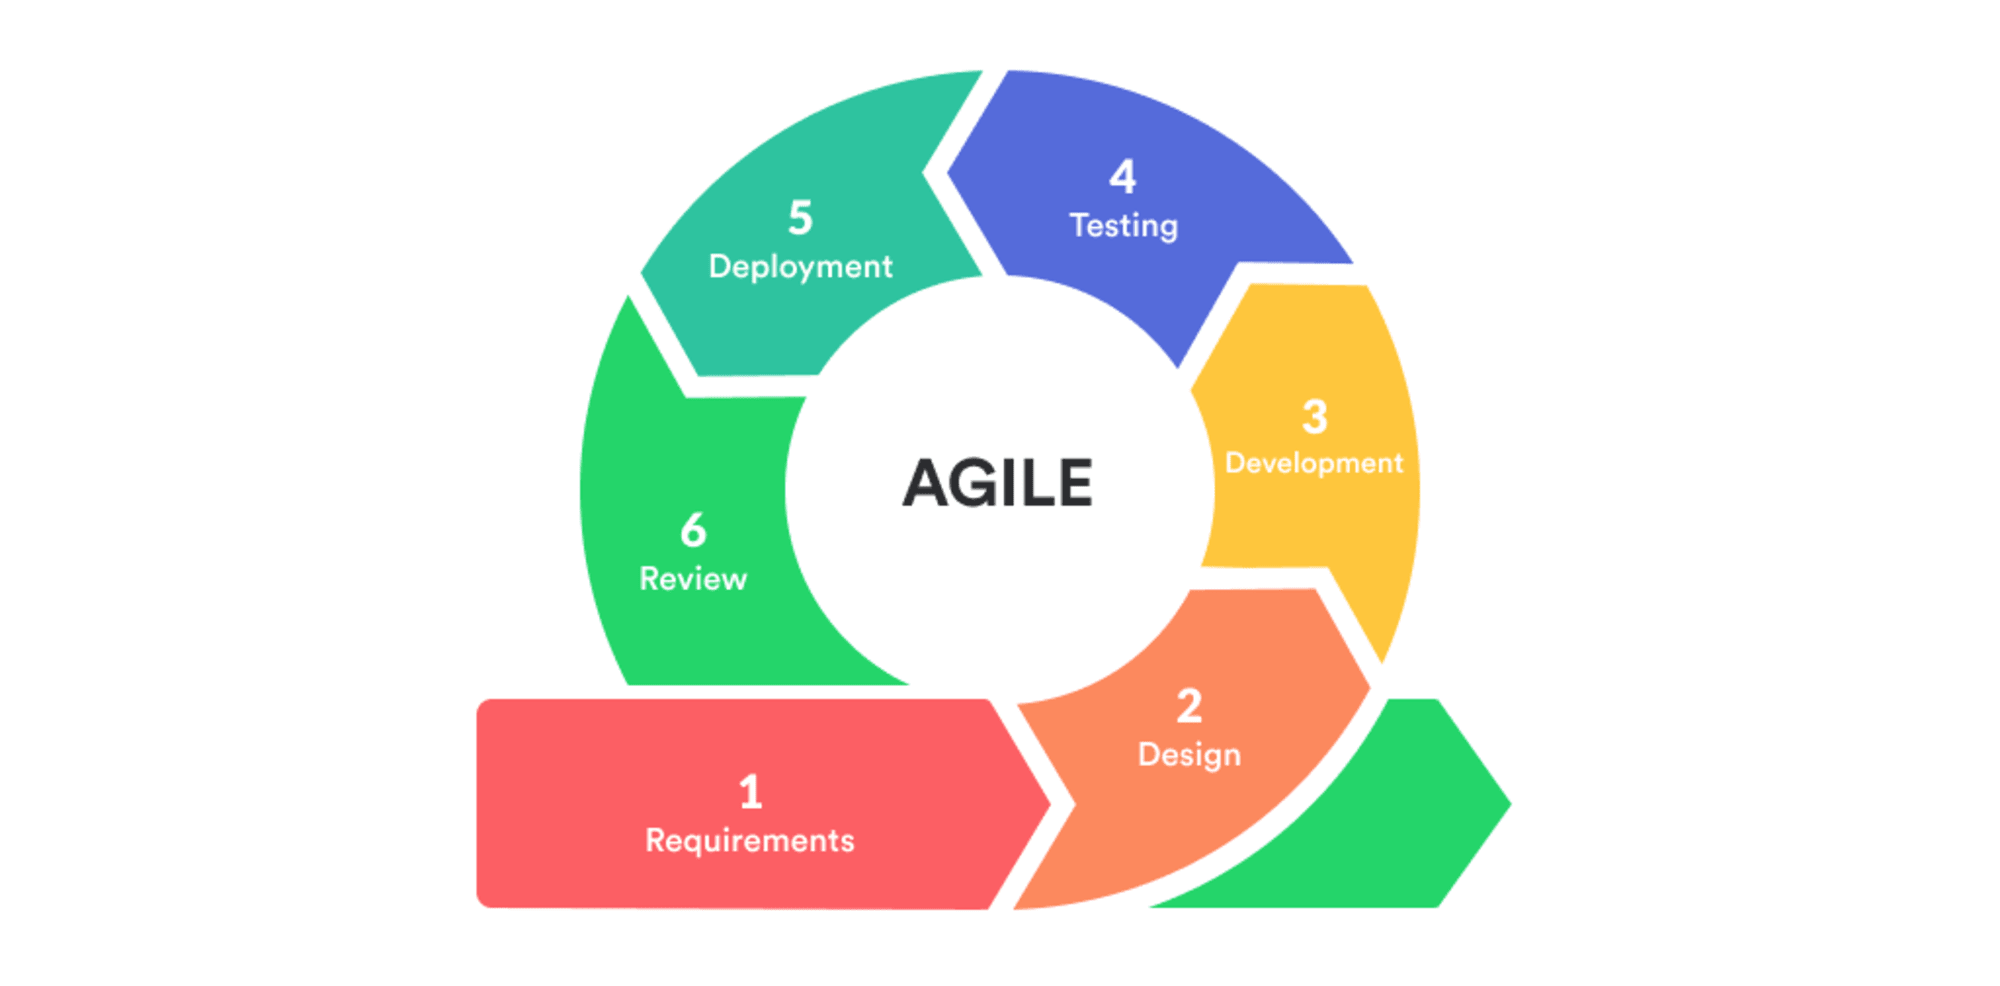
\includegraphics[width=0.8\linewidth]{figures/agile.png}
  \caption{Agile methodology.}
\end{figure}
\vspace{0.5cm}

In our project, we focus on successful implementation from the moment of initiation to the MVP (Minimum Viable Product) \cite{mvp} of the product, we focus on the philosophy of flexible project management, an agile methodology \cite{agile} that promotes better adaptation to various changes during the project. 
Let us figure out a little about agile \cite{agile}. This is a philosophy of flexible project management philosophy that promotes rapid adaptation to changes, as well as a modern approach in which the team works together with the customer to determine the needs of the project. \textbf{There are also 4 principles of the Agile Manifesto:} \cite{agilemanifesto}:

\begin{enumerate}
\item People and interaction are \textbf{more important} than processes and tools.
\item A working product is \textbf{more important} than comprehensive documentation.
\item Cooperation with the client is \textbf{more important} than agreeing on the terms of the contract.
\item Being ready for change is \textbf{more important} than following the original plan. 
\end{enumerate}

At the beginning of the our project, we conducted some kind of brainstorming, then highlighted this project idea, then we were engaged in creating project documentation, and this is the project charter plan \cite{projectcharter}, Gantt chart \cite{gantChart}, communication plan \cite{communicationplant}, split our work into 15 weeks in we call as sprints, in each 1 week for to do tasks, used the SCRUM \cite{scrumguide} framework, project execution plan \cite{executionplan}, RACI Chart \cite{racichart}, who is responsible for what - SWOT analysis chart \cite{swotanalyse} what are the strengths and the weaknesses of the team, the risks \cite{risksanalyse}, and the analysis of stakeholders. We also called once every 3-4 weeks by discord \cite{discord} and telegram \cite{telegram} to support the plan and discuss the project. Also, during the project, we created a product backlog in JIRA using the KANBAN board \cite{jira} and worked through this application. After one sprint, we conducted a task test to identify bugs also we played in scrum poker for identify for speed for each tasks in story point which means that how many days to do task need to.

\section{Scrum + Kanban}\label{scrmkan}
\begin{figure}[ht]\label{fig:kanbanboard}
  \centering
  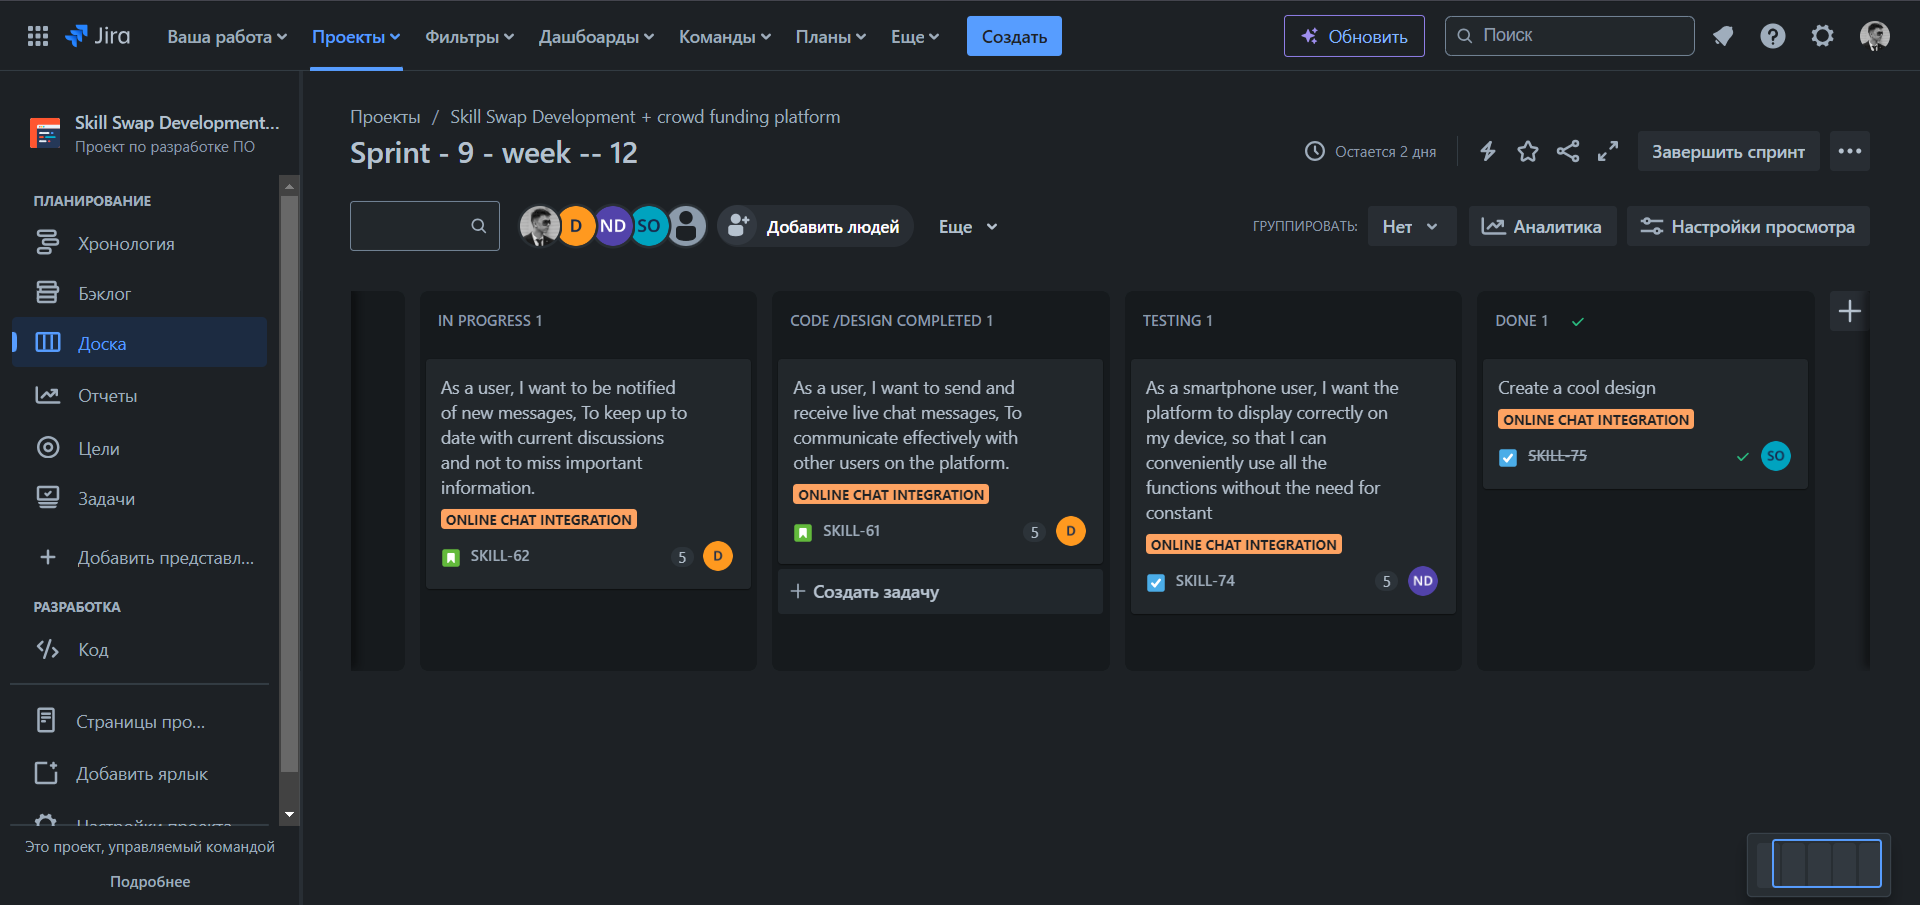
\includegraphics[width=0.8\linewidth]{figures/Kanban board.png}
  \caption{Scrum sprint + Kanban board.}
\end{figure}

 Agile philosophy \cite{agile} has its own frameworks, the most popular of them is Scrum + Kanban \cite{jira}. We worked on framework which name is scrum, that is, we determined what values the team had and also determined the team's responsibilities. In this case, our team turned into a cross-functional one. Let's take a little look at what a scrum is \cite{scrumguide}. Scrum is a lightweight framework that helps people, teams, and organizations create value through adaptive solutions and to solve complex problems. \textit{Components:} An iterative approach with a team of up to 10 people working in sprints (1 (2) - 4 weeks). Scrum clearly defines values, roles, and procedures that will help employees focus on repetitive work and its continuous improvement.\textbf{Team roles in the scrum team \cite{scrumguide}:}

\begin{itemize}
    \item \textbf{Scrum Master} - ensures compliance with processes in our case this is  (Project Manager).
    \item \textbf{Product owner} - defines the requirements for the product (Our diploma instructor).
    \item \textbf{Developers} - implement the product (team). 
\end{itemize}

Now to kanban \cite{kanban}, this is a visualization method that gives additional motivation to accomplish the goal of kanban itself, the board is divided into: 

\begin{itemize}
    \item \textbf{To Do} - what should we to do with our project. For example: As a user, I want to easily navigate the main page, so that i can understand the purpose and features of the platform.
    \item \textbf{In process} - what currently develop 
    \item \textbf{Testing} - if task complete by full - stack developer then Quality Assurance test their work.
    \item \textbf{Done} - after test if all is well then this work is complete.
    
\end{itemize}

\section{Business analytics our team}\label{bussanl}
\hspace*{0.5cm} On the basis of the preliminary analysis, we have started the project implementation process. To do this, we have distributed roles and responsibilities in the following order for be a cross-functional team:

\begin{itemize}
    \item Ossipov Alexandr - 200103001@stu.sdu.edu.kz, Team lead Project Manager. 
    \item Daulet Lepessov  - 200103213@stu.sdu.edu.kz, Full-Stack - developer. 
    \item Nurlan Darzhanov - 200103481@stu.sdu.edu.kz, IOS - developer. 
    \item Saya Oryskhan  - 200103459@stu.sdu.edu.kz, UX/UI + Quality Assurance.  
\end{itemize}

Now let's take a closer look at what each team member was doing. Let us start with the \textbf{first member} of the team with the project manager and team leader, \textit{Alexandr Ossipov}. In the course of this work, a lot was done: We divided the project into 4 parts, and this is the moment.

\begin{enumerate}
    \item \textbf{Initiations} - Brainstorm read diploma in structure. 
    \item \textbf{Planning} - Create plan for this project deadlines and etc. 
    \item \textbf{Execution and documentation} - Execute project by documentation. 
    \item \textbf{Closing the project} - writing a thesis and deploying our product.
\end{enumerate}

 Further, during this project, he organized online discord \cite{discord} and telegram meetings \cite{telegram}, monitored the quality of sprints and deadlines, motivated each team member for the successful implementation of various tasks, did some brainstorming prototyping the application and website together with the team at the initial stage of the project. We also created various documentation: the project charter \cite{projectcharter}, the project execution plan \cite{executionplan}, and so on. All links in the following are attached in references part. 
\vspace{0.5cm}
\par
\textbf{The second member} of the team is our full-stack developer \textit{Daulet Lepessov}. During this project, he was a key member of the team since our main application is a website. During the execution, he did a lot of work, wrote more than one thousand lines of code for the excellent operation of the application, followed strict deadlines, used the laravel \cite{laravel} framework with the PHP programming language, this was the \nameref{back} part. He also did \nameref{front} work, wrote a visual of the site, and used node for design, using frameworks: REACT.JS \cite{react} + HTML + CSS + JS\cite{htmlcssjs} + bootstrap\cite{boostrap} + jQuery\cite{jquery}.
\vspace{0.5cm}
\par
Our \textbf{third team member} is also a key one, \textit{Nurlan Darzhanov}, he is our \nameref{ios} developer, he made an application for iPhones using the Swift programming language \cite{swift}. 
\vspace{0.5cm}
\par
And finally, our \textbf{fourth team member} is \textit{Saya Oryskhan}, too, she was our \nameref{des} and \nameref{qa}, she made the coolest design using UX/UI \cite{design} on that, for a web application and a phone application, all screenshots will be attached below in references part and at the end of each sprint she tested the tasks that were on each week to help developers make the product better.
    \chapter{Market Analysis}\label{ch:C}
\section{Competitive Analysis}\label{companl}
\hspace*{1cm} Nowadays, more and more students are looking for platforms that will help them share knowledge and skills, especially students who need help with examples in documentation code, and so on. Online resources such as headhunter.kz \cite{headhunter}, Stackoverflow.com \cite{stackoverlow}, Reddit.com \cite{reddit}.
They offer a wide range of job search, ask questions, answer them, and so on, which allows students to study effectively. However, there is a need for specialized platforms for university students, where they could share knowledge and support joint projects within the university in order to be more effective.The increasing interest in crowdfunding also points to the need to create a platform that will bring students together to implement their projects with the help of community support or investors. Thus, the market has the potential to develop an innovative platform that will connect university students and provide them with opportunities to share knowledge, support projects and attract funding through crowdfunding \cite{crowdfunding}, as well as ask questions by answering them, that is, create one large community.

\begin{figure}[ht]\label{fig:market}
  \centering
  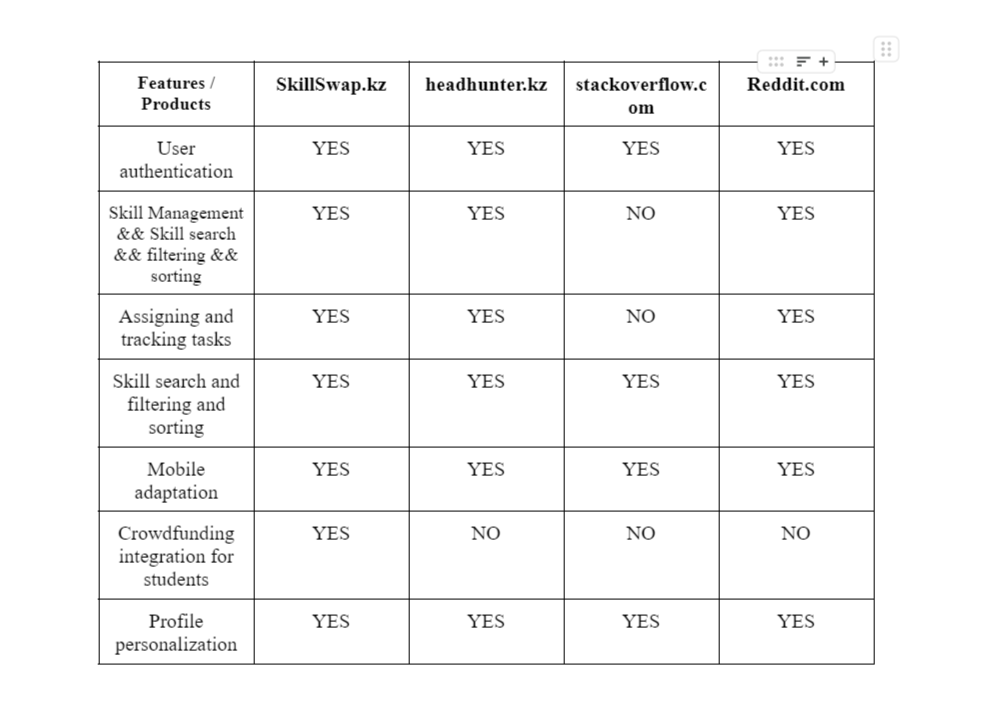
\includegraphics[width=0.75\linewidth]{figures/market analyse.png}
  \caption{Market analyse.}
\end{figure}
\newpage
\section{Product Analysis}\label{prdanl}
\subsection{Target Audience}\label{trganl}
\justifying
\hspace*{1cm} The target audience for this product according to our questionnaire, all screenshots of the questions will be provided at the end of the document this target audience from our survey \cite{survey}:
\vspace{0.5cm}
\par
Gender: Men (87.5 in percent) and Women (12.5 in percent) 
\par
Age: 16 - 18 (7.7 in percent), 19 - 21 (69.21 in percent), 22 - 25 (23.1 in percent)
\par
Status: Students (100 in percent)
\par
Location: Kazakhstan
\subsection{Target Market}\label{trgmrk}
\hspace*{1cm} The type of application that will work for our users is the B2C domain. It turns out that this will be a kind of freelance among students; self-freelance means that these are self-employment specialists who will provide their services to others for money or for free, and this scheme will work in our web application and on the phone. Determine our target market area. 
\par
We used method \href{https://www.insales.ru/blogs/university/metodika-5w-marka-sherringtona}{5 W} on that:
\par
\begin{itemize}
    \item \textit{What - What are you selling ?}
    \par
    Online platform where can students get skills which their prefer.
    \item \textit{Who - Who buys your products?}
    \par
    All students from Kazakhstan.
    \item \textit{Where — Where do you sell?}
\par Our web platform and mobile.
    \item \textit{When — When does a customer have a need for a product?}
\par When they want to get skills from another person and maybe they will be friends.
    \item \textit{Why — Why should the customer buy the product from you?}
    \par
    Basically it's gonna be a free but to get new futures and able to do donate for another person to give motivation to do the best projects in the world.
\end{itemize}
    \chapter{Implementation}\label{ch:D}
\section{Development process}\label{devprc}
\begin{figure}[ht]\label{fig:market}
  \centering
  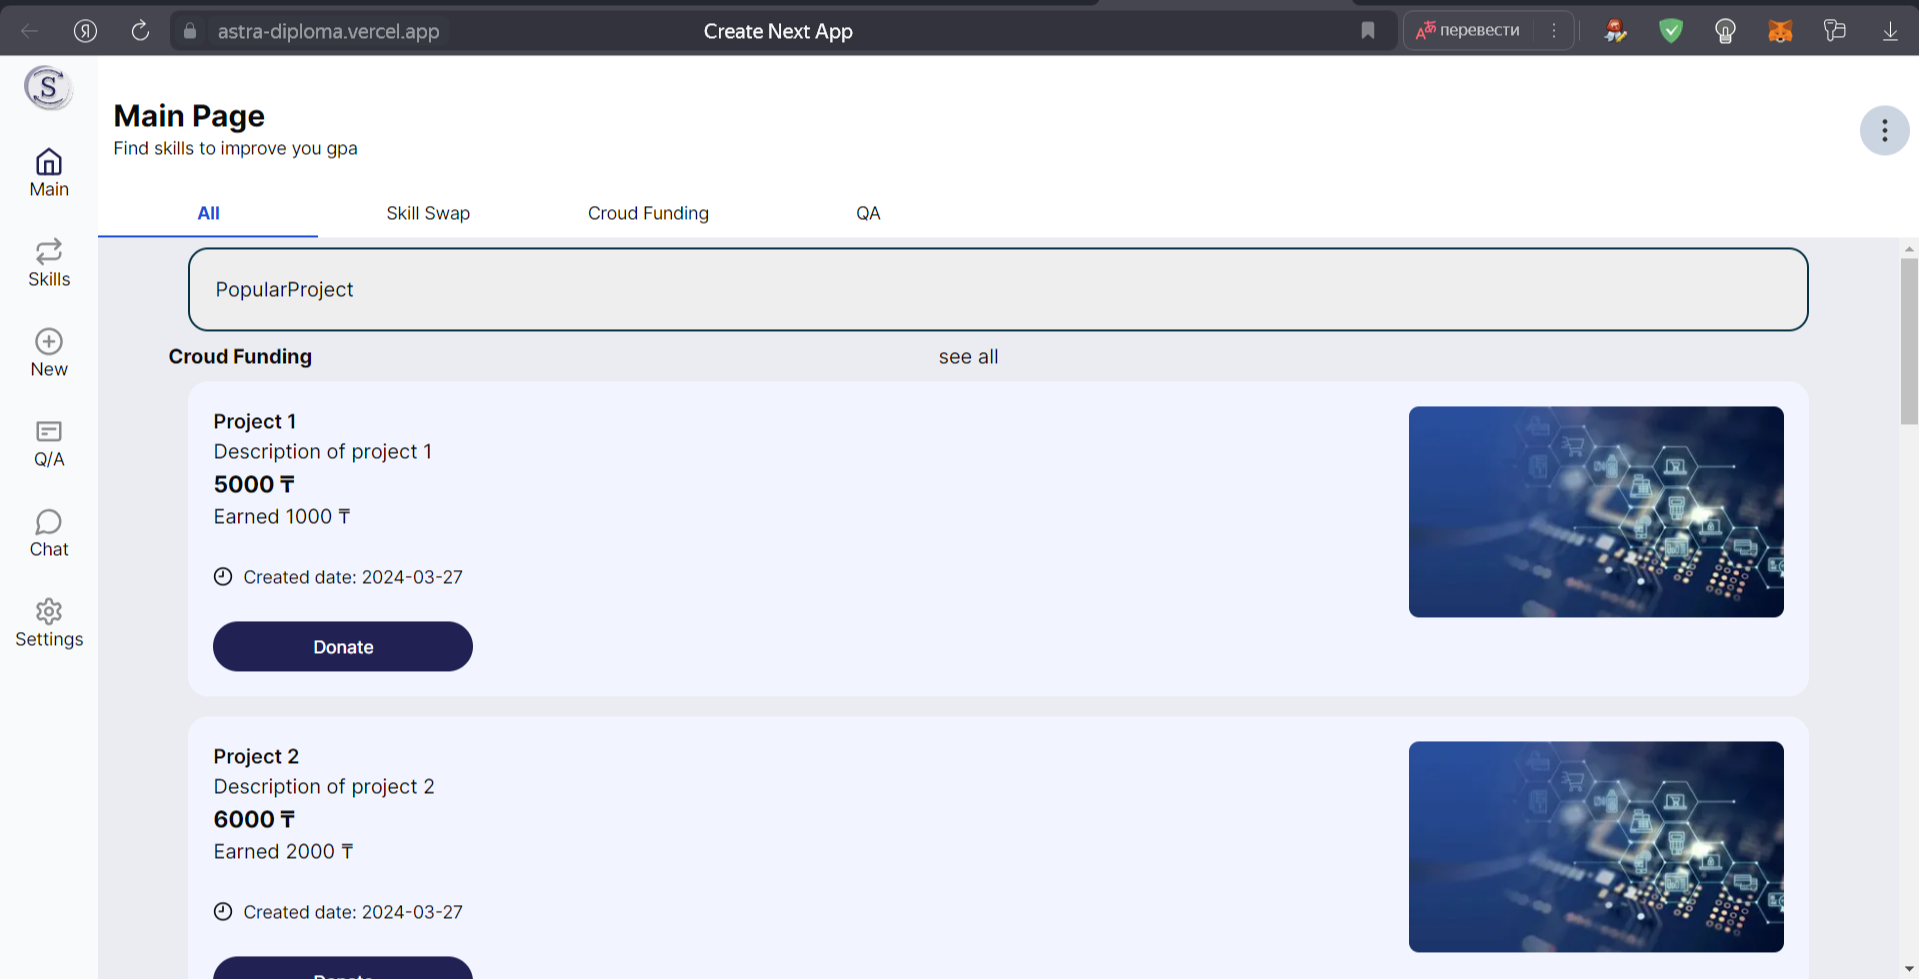
\includegraphics[width=0.8\linewidth]{figures/Website.png}
  \caption{The screenshot our website hosting on AWS \cite{aws}.}
\end{figure}

During the development of our products based on the mutually beneficial exchange of skills and not only this project was divided into some component parts: the \nameref{des} development process starting with wire-frames, pumping the main application design further UX/UI, the process of website design is underway to compile the visual part of the site for mobile adaptation \nameref{front}, beautiful animation, for better interaction on the website, further work is underway on \nameref{back} part is the development of functions for the operation of the site, and this is our registration form, login, chat, rating, user setup, responding to different skills, donation system search process, filters, sorting and much more and the most important deployment of the web hosting project on Amazon Web Service \cite{aws} \nameref{back} is also an \nameref{ios} - based application for mobile phones using the web view function as similar to its analogues kaspi.kz \cite{kaspi}. Let us take a closer look at every aspect of this project, namely web \nameref{des}, mobile development \nameref{ios}, and \nameref{qa} of this product writing test cases, as well as all screenshots the links will be attached below this document in -  \nameref{app:AA}.

\newpage
\section{User Flow}\label{usrflow}
Our user flow show \cite{miro} that the simple steps that the user performs in our application.
The purpose of this user flow \cite{miro} is to give users the opportunity to use our SkillSwap \cite{skillswap} platform in the most effective way.
\begin{itemize}
    \item \textbf{Here is the step-by-step process:}

\item The user goes to the main page of the application.
\item The user sees the website or application of the homepage where it is shared on skilswap, question answer crowd funding.
\item In order to use the platform, the user must register on the website in order to use the platform by choosing a student or an ordinary user.
\item After registration, the user can use the platform if the student all sections are available since this is a student-only platform. If a regular user, then only crowd funding is available.
\item The user can chat, ask questions, answer them, and so on. 
\item There are also settings where he can configure what number, mail, and so on he wants. 
Branching paths:
\item \textbf{Invalid email address:}
\item If the format of the email address is incorrect, an error message is displayed.
The user is prompted to enter a valid email address.
\end{itemize}

\begin{figure}[ht]\label{fig:userflow1}
  \centering
  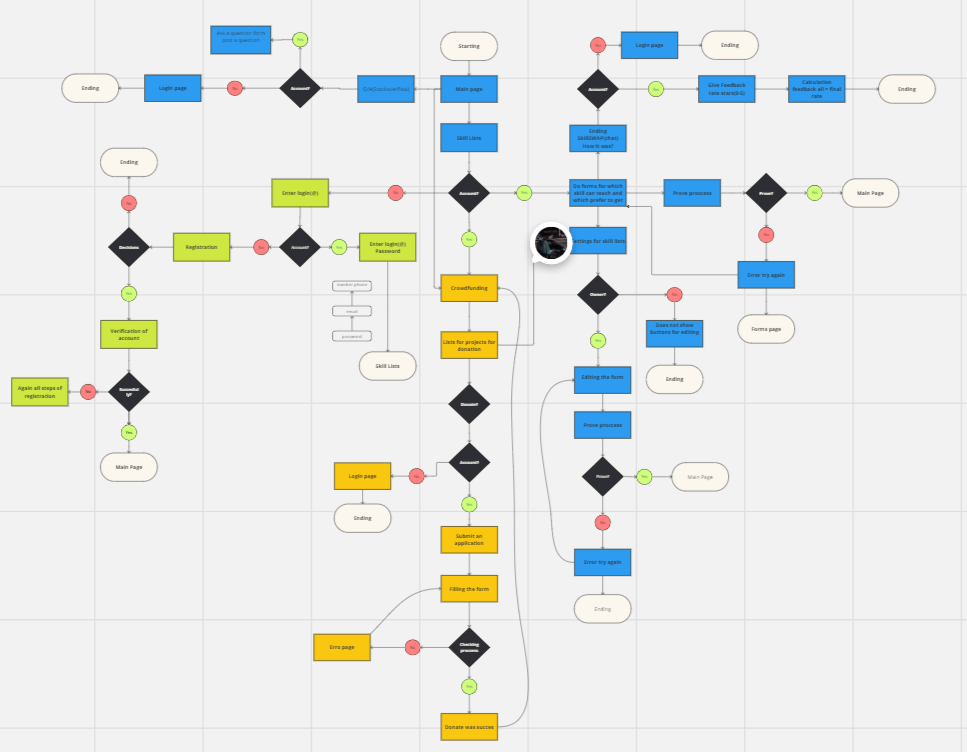
\includegraphics[width=0.8\linewidth]{figures/Userflow - 1.png}
  \caption{First type of userflow.}
\end{figure}

\begin{figure}[ht]\label{fig:userflow2}
  \centering
  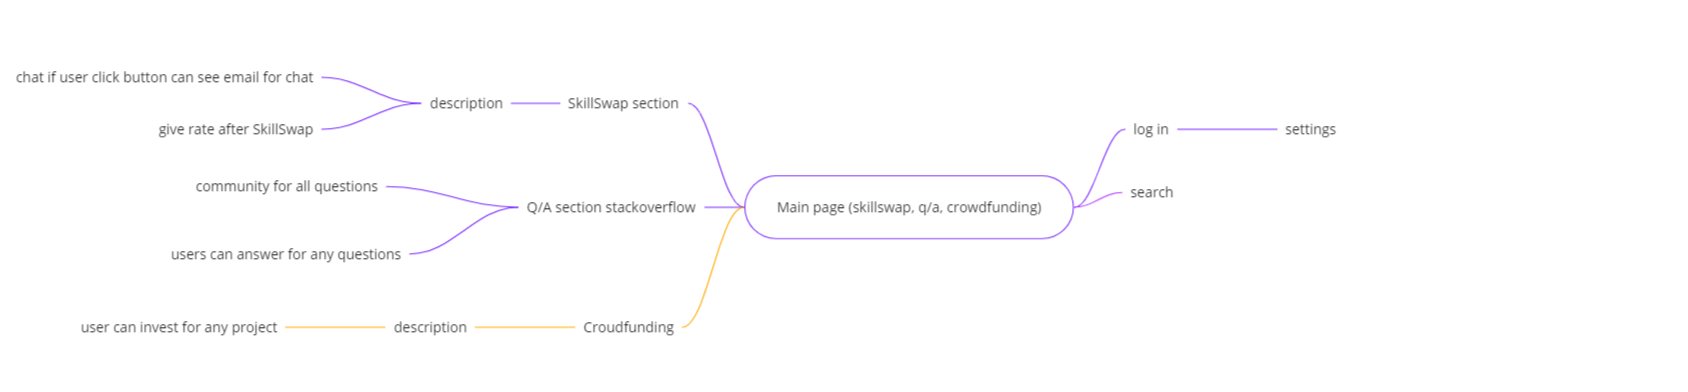
\includegraphics[width=0.8\linewidth]{figures/Userflow -2.png}
  \caption{Second type of userflow.}
\end{figure}

\newpage
\section{Implementation}\label{impl}
\subsection{Design}\label{des}
When brainstorming ideas about the \nameref{des} of our project, we concluded that we wanted to keep it simple, modern, and easy for users to navigate. So, we reached two main conclusions: choosing the right color to represent the entire project and prioritizing User Experience (UX) \cite{design} components.

First, we defined the placement of buttons, how to display warnings, etc., to ensure a meaningful and relevant experience for users. Then, I created a wireframe \cite{wireframe}, which underwent several changes after each meeting with the team and with every new functionality change in our project.

\begin{figure}[ht]\label{fig:wireframe}
  \centering
  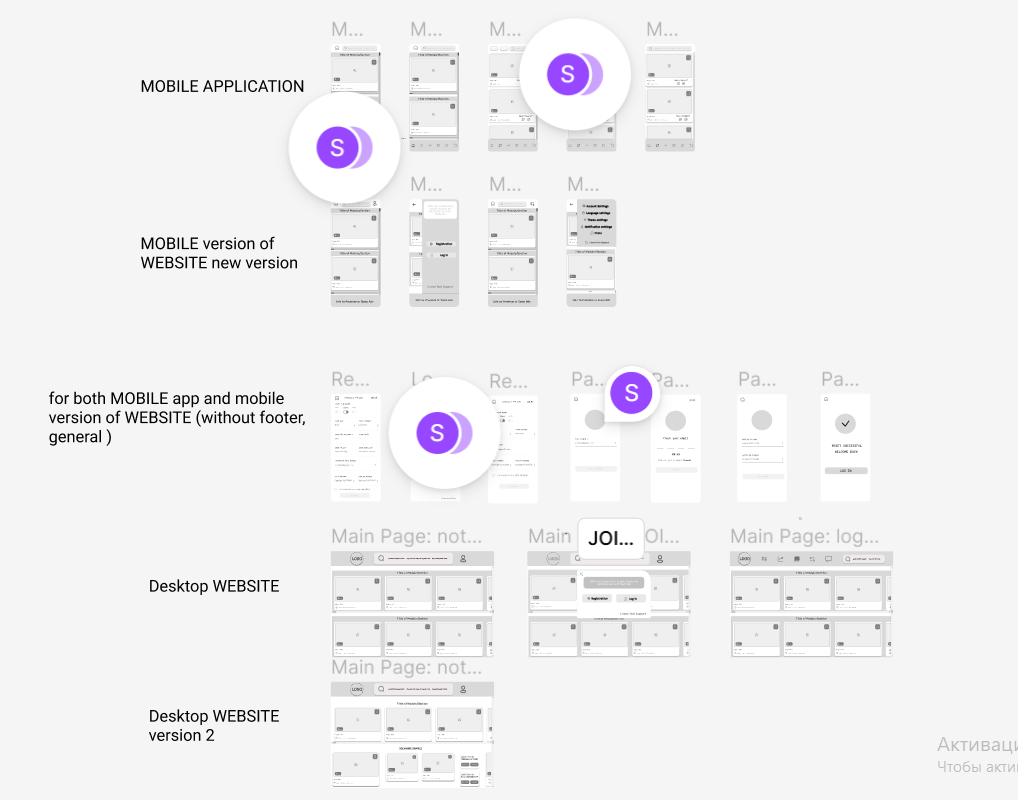
\includegraphics[width=0.8\linewidth]{figures/wireframe.png}
  \caption{The screenshot of our wireframe.}
\end{figure}

The most significant aspect for us was choosing the main color of our platform. Since our project is directly related to students, we were inspired by the representative color of our university, which is Dark Sapphire \textit{(082673)}. As we associate the university's color with tradition and honor, we decided to retain it and introduce innovation by incorporating a darker shade, resulting in Space Cadet \textit{(212153)} as our primary color. 

\begin{figure}[ht]\label{fig:colors}
  \centering
  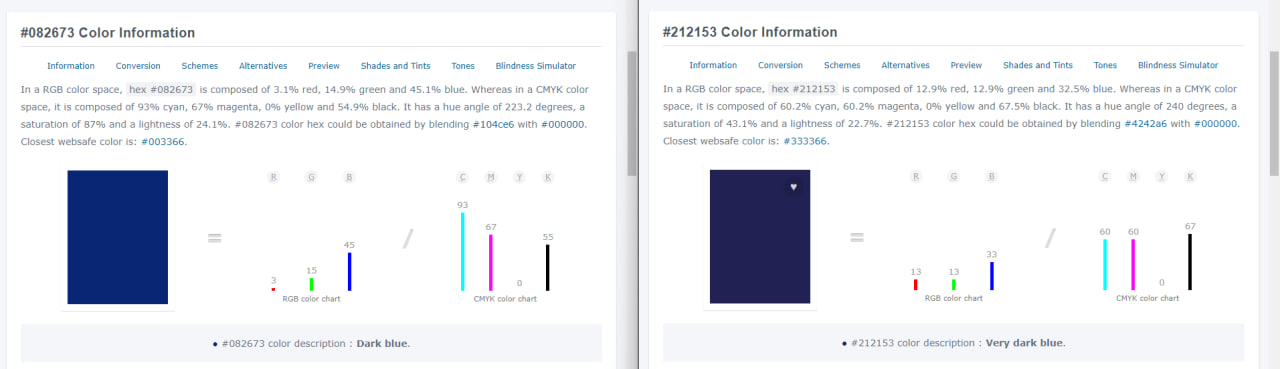
\includegraphics[width=0.8\linewidth]{figures/color comparison.jpg}
  \caption{The screenshot of comparison: University color, our project's color .}
\end{figure}
\newpage
Other colors in our project were chosen to be simple derivatives of the main color, along with gray, white, and black to maintain a classic appearance. As a result, we have achieved a \textit{minimalistic and comfortable} platform for future users.

\subsection{Frameworks}\label{frmw}
Decision to make Laravel \cite{laravel} the main framework for this project because of several advantages it offers. Firstly, Laravel \cite{laravel} is popular for its efficiency, what makes it perfect fit for small or medium sized web-applications, which is well-suited for our project requirements. One of the best advantages of the framework is robust debugging tool and many good libraries, which helps a lot during developing process and efficient issue resolution.
Routing system. Laravel \cite{laravel} has good and simple routing system, it simplifies the maintaining of applications routes and enhances overall code readability.Large community. Laravel \cite{laravel} has a large and active community, which proves invaluable when faced with complex challenges during development
Overall, Laravel \cite{laravel} current state as one of the most used and maintained framework ensures continuous support, regular updates, and security patches, contributing to the long-term stability and reliability of our project.
\par

\hrulefill 

To work on  \nameref{ios} we used a UI framework provided by apple themselves in 2019 - SWIFT UI \cite{swift}, which allows you to create dynamic and beautiful user interfaces with minimal effort. 

\textbf{Creating views} - We defined different views using Swift UI \cite{swift} declarative approach. Each view constitutes a separate component of the interface and can be easily adapted and reused.

\textbf{Modular architecture} - We have broken the application into small modules, each containing a set of views and functions for specific functionality. This makes the code more readable and maintainable.
For example, the screenshot below clearly shows us that we separated the UI element in the form of a sheet and built it separately so that the code would be cleaner and clearer in the whole file.

\begin{figure}[ht]\label{fig:screenios}
  \centering
  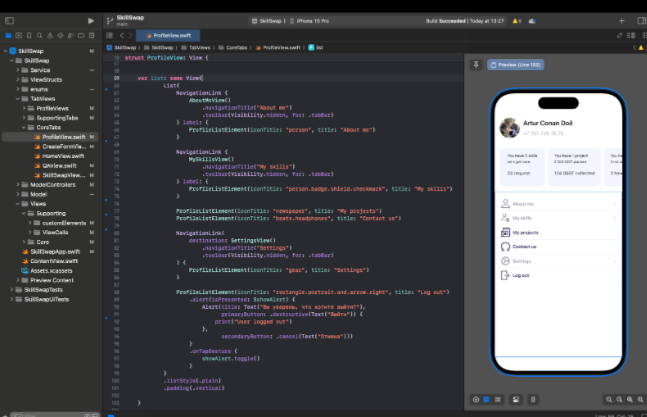
\includegraphics[width=0.8\linewidth]{figures/Screen IOS.png}
  \caption{The screenshot of our IOS application.}
\end{figure}

\subsection{Front-tend}\label{front}

For the React framework \cite{react}, we chose it as the main \nameref{front} \cite{htmlcssjs} framework for several reasons. \textbf{Firstly}, React \cite{react} is renowned for its efficiency, making it an ideal choice for developing small - to medium-sized web applications, which aligns perfectly with the scope of our project. Additionally, React \cite{react} boasts a powerful debugging tool and a vast array of libraries, facilitating smoother development processes and quicker issue resolution.
React \cite{react} component-based architecture offers a streamlined approach to building user interfaces, promoting code reusability and enhancing maintainability. This modular structure simplifies the development of complex applications by breaking them down into manageable components.
Furthermore, React \cite{react} benefits from a large and vibrant community of developers who actively contribute to its ecosystem. This extensive community support provides invaluable resources, including tutorials, documentation, and third-party libraries, which expedite development and troubleshooting processes. \textbf{Lastly}, React \cite{react} status as one of the most widely used \nameref{front} frameworks ensures continuous updates, feature enhancements, and security patches, bolstering the long-term stability and reliability of our project.

\subsection{Back-end}\label{back}
During the development of the \nameref{back} of our web application, we prioritized the adherence to the Object-Oriented Principles (OOP), including reusability, inheritance, and encapsulation.

We also followed the SOLID principles, which guided our design decisions throughout the development process. Specifically, we focused on:

Single Responsibility Principle: Each class or module had a single responsibility, promoting code maintainability and reducing coupling between components.
Open/Closed principle: Our code was designed to be open for extension but closed for modification, allowing for future enhancements without altering existing code.
Dependency Injection: We utilized dependency injection to invert the control of dependencies, making our code more modular, testable, and flexible.
Additionally, we aimed to keep our code DRY (Don't Repeat Yourself) \cite{dry} and KISS (Keep It Simple, Stupid) \cite{kiss}. By avoiding code duplication and complexity, we improved readability, maintainability, and debugging efficiency. In terms of design patterns, we leveraged middle ware, inspired by the Chain of Responsibility pattern, to handle common cross-cutting concerns such as authentication, logging, and request/response manipulation.

Of course, the above patterns and rules we also used for our project abstractly and we tried our best to keep them.

\newpage
\subsection{Models}\label{modls}
Data models are created to work with the API, to transform the data we receive into a form that is understandable for our app. On \nameref{ios}, we use four main types of models:
\begin{enumerate}
    \item \textit{Authorization models} - represent the data required for the user authentication process in an application. In our application, we use two models for this purpose: 
    \item \textit{Registration model} - contains the data required to register a new user such as email, password and other required attributes. Authorization model: contains the data required for registered users to log in to the system, such as email and password.
    \item \textit{Skills Sharing Model} -  The skill sharing model represents data related to the ability of users to share their skills and services within the application. This model contains information about the user offering their skill and the user looking for the corresponding skill.
    \item \textit{Crowdfunding model} - The crowdfunding model contains data about projects that require funding from the user community. This model includes information about the project, its goals, timeline, amount of funds needed, and current fundraising status.
    \item \textit{Question and Answer (QA) Model} - the QA model is used to represent information about the questions asked by users and their corresponding answers within our application. This model contains the text of the question, a list of answers, and metadata such as the date the question was created and the number of views. This all screenshot in below in \nameref{app:BB} part
\end{enumerate}

\subsection{Views}\label{views}
In this part of our development, we utilized various \nameref{front} tools to create an engaging and dynamic user experience:

React \cite{react} Components: Our \nameref{front} is built using React \cite{react} components, which provide a modular and reusable approach to building user interfaces. Additionally, React \cite{react} enables us to create interactive and responsive user interfaces, with data being dynamically updated as users interact with the application.

CSS (cascading style sheets) Styling \cite{htmlcssjs}: We used CSS stylesheets to define the presentation and layout of our application's UI elements. We used CSS \cite{htmlcssjs} frameworks such as Bootstrap \cite{boostrap} to streamline the styling process and ensure consistency across our application.

JavaScript \cite{htmlcssjs}: JavaScript played a crucial role in enhancing interactivity and functionality in our \nameref{front}. We utilized JavaScript libraries and frameworks like Axios to make asynchronous HTTP requests to our \nameref{back} API. This enabled us to retrieve and update data from the server without reloading the entire page, resulting in a smoother and more seamless user experience.

\par
\hrulefill 

Our \nameref{ios} application consists of several blocks such as:
\begin{itemize}
    \item \textit{Welcome Screen} - The Welcome Screen is where users are greeted with a brief description of our application's functionality. This screen, like a curtain, is a business card that gives a fleeting glimpse of how our application can be used.
    \item \textit{Registration Screen} - After first launching the app, users are taken to the registration screen where they can create their unique account. This step allows users to access all of the app's features, opening up a world of new possibilities.
    \item \textit{Authorization Screen} - For registered users, an authorization screen is available where they can log into their account using pre-created credentials. This step provides quick and secure access to the personal account and personalized features.
    \item \textit{MainTabView} - The Home screen is the control center for all major functions of the application. It provides a navigation hub through which users can freely navigate through the different sections of the app. Here are some of the key SubViews and HomeView: This section gives the user access to current news, updates and interesting events within the application.
    \item \textit{Skill Sharing (SkillSwapView)}: This is where users can find other users to share skills, services and knowledge.
    \item \textit{Create Post View:} This section allows users to create and publish their own posts and share information and ideas with the community.
    \item \textit{QA (QAView)}: Here users can ask questions and get answers from other community members, enriching their knowledge and experience.
    \item \textit{Profile View:} This section allows users to manage their profile, customize settings, and view their activity in the app.
    \item \textit{The MainTabView} is the main hub of user interaction with our application, providing many opportunities for users to explore, communicate, and learn.
\end{itemize}

\subsection{Forms}\label{forms}
\begin{enumerate}
    \item \textbf{Registration Purpose: Register new users to access the application functionality.}
\begin{itemize}
    \item Form fields:
    \item Email
    \item Phone number
    \item First Name
    \item Last name
    \item Password
\end{itemize}
\textbf{Actions:} Once the form is filled out, the user's data is saved in the database and the user is able to log in using their credentials.

\par
\vspace{0.5cm}

\item \textbf{Authorization Purpose: To confirm the user's identity for access to the personal account.}
\begin{itemize}
\item Form fields:
\item Login (email or phone number)
\item Password
\end{itemize}
\textbf{Actions:} After filling out the form, the data is checked for compliance with the data in the database, and in case of successful authentication the user gets access to the personal account.

\par
\vspace{0.5cm}

\item \textbf{Creating a post (Skill Swap)Purpose: To publish skill swap offers with other users.}
\begin{itemize}
    \item Form fields:
    \item Title
    \item Description (content)
    \item Photo (optional)
\end{itemize}
\textbf{Actions:} Once the form is filled out, the post is displayed on the platform where other users can see it and react.

\par
\vspace{0.5cm}

\item \textbf{Create a post (Crowdfund)Purpose: To raise funds for a specific project or product.}
\begin{itemize}
\item Form fields:
\item Product/project name
\item Description (content)
\item Amount raised
\item Planned amount
\item Photo (optional)
\end{itemize}
\textbf{Actions:} Once the form is filled out, the project is displayed on the platform where other users can see it, donate, and track fundraising progress.

\par
\vspace{0.5cm}

\item \textbf{Create a post (Question)Purpose: To ask questions and get answers from other users.}
\begin{itemize}
    \item 
Form Fields:
\item Title
\item Question (content)
\item Photo (optional)
\end{itemize}
\textbf{Actions:} After filling out the form, the question is displayed on the platform where other users can see it and leave answers.
\end{enumerate}


\subsection{IOS}\label{ios}
 The \nameref{ios} application gives users convenient access to your service functionality on Apple devices, allowing them to interact with the community, share skills, and create new opportunities.System Requirements: Supports \nameref{ios} version 13.0 or higher. Internet connection is also required for the app to work. Install and Run: Users can install it on their devices using the App Store or join the beta testing through TestFlight \cite{testflight}. \textit{User Interface}: The application interface is friendly and intuitive. Users can easily create posts, search for skills or ask questions using simple and straight forward controls. \textit{Application functionality:} Users can register, log in and create posts in various categories such as SkillSwap \cite{skillswap}, Crowdfund and Questions. The app provides the ability to share skills, fundraise for projects and ask questions to the community. \nameref{back} and \nameref{front} integration: The application interacts with the \nameref{back} and \nameref{front}, providing data transfer and request processing via API.

\section{Quality Assurance}\label{qa}
The testing process of our project began with the implementation of the \nameref{front} carcass. As the \nameref{qa}, we initiated the creation of basic UI test cases to ensure the visual correctness aligns with the approved design by our team. Once the \nameref{back} was implemented and integrated to the \nameref{front} end by our developer, It was decided to provide end-to-end testing to ensure effective validation of each functionality. Meaning of end-to-end testing is conducting tests to every possible user interaction, from registration to login and beyond, across the entirety of the platform. Subsequently, We conducted mobile testing to assess the platform's responsiveness. Finally, User Acceptance Testing (UAT) was carried out, marking the concluding phase of testing overseen by me. Additionally, routine code reviews and smoke tests were conducted by both our developers and the project manager to ensure quality and functionality

\section{Architecture}\label{arch}
The project is a web application designed to facilitate communication and collaboration between students, allowing them to create posts, ask questions, and participate in skill-based exchanges.
\begin{enumerate}
    \item \textbf{\nameref{front} Architecture}
\begin{itemize}
    \item The \nameref{front} of the application is built using React.js \cite{react}, a popular JavaScript \cite{htmlcssjs} library for building user interfaces.
    \item \textbf{Components:} The \nameref{front} consists of modular components that handle various aspects of the user interface, such as posts, questions, skill funds, and user profiles.
    \item \textbf{State Management:} Redux is used for state management, allowing for centralized management of application state and data flow.
    \item \textbf{Communication with \nameref{back}} : The \nameref{front} communicates with the \nameref{back} REST full API to fetch and update data using asynchronous HTTP requests.
\end{itemize}

\item \textbf{\nameref{back} Architecture}
\begin{itemize}
    \item \nameref{back} part of our web-application was written using Laravel \cite{laravel}.
    \item The \nameref{back} gives access for multiple API endpoints allowing CRUD operations for skillswaps, skillfunds and questions with their answers.
    \item Authentication and authroization is implemented by middlewares, ensuring that only authenticated users can access certain endpoints.
    \item \nameref{back} interacts with relational database (PostgreSQL) \cite{postgressql} to store information related to posts, questions, users, and their interactions.
\end{itemize}

\item \textbf{Logging}
\begin{itemize}
    \item Web-application logs every info, error and warnings into its default log system.
\end{itemize}

\item \textbf{Security}
\begin{itemize}
    \item Authorization and authentication protect application from common threats.
    \item User authorization handled by laravel \cite{laravel} sunctum, given users token for further access for our endpoints.
    \item Input validation for CRUD and other operations, prevents our application from SQL \cite{postgressql} injections.
\end{itemize}

\item \textbf{Deployment Architecture}
\begin{itemize}
    \item Application is deployed by Amazon Web Service \cite{aws}.
\end{itemize}
\end{enumerate}

\section{Databases}\label{dbms}
 The project uses PostgreSQL \cite{postgressql} as the database management system (DBMS) \cite{dbms} due to its robust features, support for complex data types, and strong emphasis on data integrity.PostgreSQL \cite{postgressql}is an open-source RDBMS known for its reliability, extensibility, and compliance with SQL standards.
 The use of PostgreSQL \cite{postgressql} allows for the efficient storage and retrieval of structured data, enabling the application to handle large volumes of information while maintaining data consistency and reliability.
 
\begin{enumerate}
    \item \textbf{Database Schema}
\begin{itemize}
    \item The database schema is designed to reflect the application's data model, which includes entities such as users, posts, questions, skill funds, categories, and ratings.
    \item Each entity is represented by a table in the database \cite{dbms}, with columns corresponding to the entity's attributes.
    \item Relationships between entities are established using foreign key constraints, ensuring referential integrity and enforcing data consistency.
    \item The database \cite{dbms} schema is optimized for efficient querying and data retrieval, with appropriate indexing and normalization techniques applied to improve performance.
\end{itemize}

\textbf{The database \cite{dbms} schema consists of the following tables:}

\vspace{0.5cm}
\par
\item \textbf{Students Table}

\begin{itemize}
\item \textit{The students} table contains primary information about students, including their name, course, phone number, university, specialty, etc.
\end{itemize}

\item \textbf{Universities Table}
\begin{itemize}
\item \textit{The universities} table stores information about all universities in the country. It includes columns for the university's name and code.
\end{itemize}

\item \textbf{Faculties Table}
\begin{itemize}
\item \textit{The faculties} table contains information about faculties within universities. This table establishes a one-to-many relationship with universities.
\end{itemize}

\item \textbf{Specialties Table}
\begin{itemize}
\item \textit{The specialties} table holds information about all specialties offered within faculties, it establishes a one-to-many relationship with faculties.
\end{itemize}

\item \textbf{Posts Table}
\begin{itemize}
\item \textit{The posts} table allows students to create, update, and delete posts. Each post can have an associated application functionality, where students can apply for a post to buy or exchange skills. The table includes columns for description, image, title, and status.
\end{itemize}

\item \textbf{Questions Table}

\begin{itemize}
\item \textit{The questions} table enables students to create and answer questions. Each question can be rated on the basis of its quality and the students can also provide answers. The table includes columns for title, question, image, and rating.
\end{itemize}

\item \textbf{Skill Funds Table}

\begin{itemize}
\item \textit{The skill funds} table is designed for students to share their startup ideas. Students can earn money if their idea gains enough popularity and support. The table includes columns for description, title, and status.
\end{itemize}
\end{enumerate}
\textbf{Cache}

In our application, we used caching to improve performance and reduce database \cite{dbms} load. Caching helps store frequently accessed data in memory, allowing for faster retrieval and response times.
\vspace{0.5cm}
\par
\textbf{We employed caching in various parts of the application, such as:}

\begin{itemize}
    \item \textbf{Database Query Results}: We cached the results of frequently executed database queries to avoid redundant database calls and speed up data retrieval.
    
    \item \textbf{API Responses}: We cached API responses to reduce latency for subsequent requests and improve overall API performance.
    
    \item \textbf{View Fragments}: We cached rendered views or view fragments to enhance the responsiveness of the application and reduce server-side processing time.
\end{itemize}

By leveraging caching mechanisms, we were able to optimize the performance of our application and deliver a smoother user experience.

\section{Additional tools}\label{tools}
\textbf{Swagger \cite{swager}}

\begin{itemize}
\item Swagger \cite{swager} was used for providing user-friendly interface for \nameref{front} and mobile developer \nameref{ios}. Our REST API \cite{rest} endpoints was documented and visualized using this technology.
\end{itemize}

\textbf{Amazon Web Services (AWS) \cite{aws}}
\begin{itemize}
    \item  We used AWS \cite{aws} for deploying our web-application.
\end{itemize}

\begin{itemize}
\item \textbf{Amazon EC2 (Elastic Compute Cloud)}: EC2 instances allowed to host and run our application.
    
\item \textbf{Amazon Route 53}: Route 53, AWS highly available and scalable DNS web service, was used for domain registration, routing traffic to our application resources, and managing domain health checks and failover configurations. It ensured reliable and efficient DNS resolution for our web applications.
\end{itemize}

\textbf{Vercel \cite{vercel}}
\begin{itemize}
\item Vercel \cite{vercel} was used to deploy our front-end part.
\end{itemize}
\textbf{Git / Github \cite{github}}
\begin{itemize}
\item members and enabling versioning, code review, and issue tracking throughout the development process. It provided a centralized repository for our codebase, ensuring visibility, traceability, and code integrity.
\end{itemize}

\hrulefill 
\vspace{0.5cm}
\par
In our \nameref{ios} application, we have chosen the MVVM (Model-View-ViewModel) architectural pattern to organize the code. MVVM offers a solution to structure the application by dividing it into three main components: model (Model), view (View) and view model (ViewModel).Why we chose MVVM: Separation of Responsibilities: MVVM helps us to clearly separate the business logic (Model), the UI mapping (View) and the interaction logic between them (ViewModel).
\vspace{0.5cm}
\par
\textbf{Ease of testing:} By separating the code into separate components, we can easily test each part independently. The view model can be tested with unit tests without having to run the UI.
Support for multiple interfaces: MVVM makes it easy to create different user interfaces such as for mobile devices, web applications or desktop applications using the same presentation model.
\vspace{0.5cm}
\par
\textbf{Cleaner and clearer code:} MVVM facilitates the creation of clean and understandable code by clearly separating logic and display.
Support for bi-directional data binding: MVVM provides bi-directional data binding between the view and the view model, which makes the process of updating data on the UI easier and more efficient. Using MVVM allows us to create flexible, maintainable and easily testable applications, which improves development productivity and provides a better user experience.

    \chapter{Result}\label{ch:E}
During the final results of our graduation project, we would like to highlight several aspects of this project. 
\begin{enumerate}
    \item \textbf{Developed components of the project or under the name of their functionality:} Within the framework of our project, a platform was created for the mutually beneficial exchange of skills between students and also a donation system, including functionality for registering new users, creating profiles, searching and viewing available skills, as well as functionality for participating in the QA system and crowdfunding and giving a rating to the questions is he good or not. 
    \item \textbf{User interface \nameref{des}:} All screenshots and links below to the platform provided allow you to visually evaluate the design and functionality of the final project developed by us.
    \item \textbf{Evaluation of completed goals:} During our analysis of the results achieved during this semester, we can conclude that most of the goals set were successfully achieved. In particular, the platform has successfully implemented the main functions that ensure the exchange of mutually beneficial skills and support for students' projects.
    \item \textbf{Testing results \nameref{qa}:} Testing of the platform revealed several minor bugs that were successfully fixed before the final version of the project. Overall, the platform has shown stable operation and high performance. 
    \item \textbf{Comparison with similar platforms:} Conducting a comparative analysis with existing platforms that offer similar functionality helped to identify unique features and areas in which our platform is superior to others or requires further improvement, that is, we took 4 types of projects and implemented them in one site specifically for students.
    \item \textbf{Data Security and confidentiality:} Assessment of the security measures applied within the framework of the platform to protect user data and privacy, ensuring compliance with relevant rules and standards. 
    \item \textbf{Action Plan for the future:} Drawing up an action plan for further development and improvements based on feedback received, new industry trends and changing user needs and preferences. This may include features such as gamification elements, integration with external tools or services, and expansion to new demographic user groups or geographic regions.
\end{enumerate}
    
    \chapter{Conclusion}\label{ch:concl}
\hspace*{1cm} The main and important goal of our graduation project was to create a modern website and IOS application, geared to students on a mutually beneficial exchange of skills through which students could find new acquaintances and get the new skills they want and crowdfunding. We started this project from scratch from January to May and strictly adhered to the regulations of the interested parties. From the very beginning of our project, we began to analyze the market and found the pain in which students do not find friends at universities, do not improve their communication skills, etc. By conducting surveys of the target audience, we tried to do everything possible to make our website and application for iOS understandable and valuable. The use of modern methodologies has greatly helped in this project management, compliance with strictly tight deadlines, and the provide of meetings. As a result, it helped us to place responsibilities between us, someone was in charge of design, someone was in charge of development, and so on. We also learned how to work in a team to support each other and motivate each other. With the difficulties we faced, it was bringing our project online since we had little experience with this problem, but we did not give up and achieved our goal. The most important thing when working on our project for us was teamwork, which will become one of the indispensable and significant skills in any other IT project, because it is very difficult for one to develop an IT project, we even say it is not possible, therefore it is very important to make new acquaintances and create new startup projects, as they say, and suddenly it will shoot.
    
    \appendix
    \chapter{Chapter A}\label{app:AA}
\section{Database UML Diagram}\label{uml}
\begin{figure}[H]\label{fig:database}
  \centering
  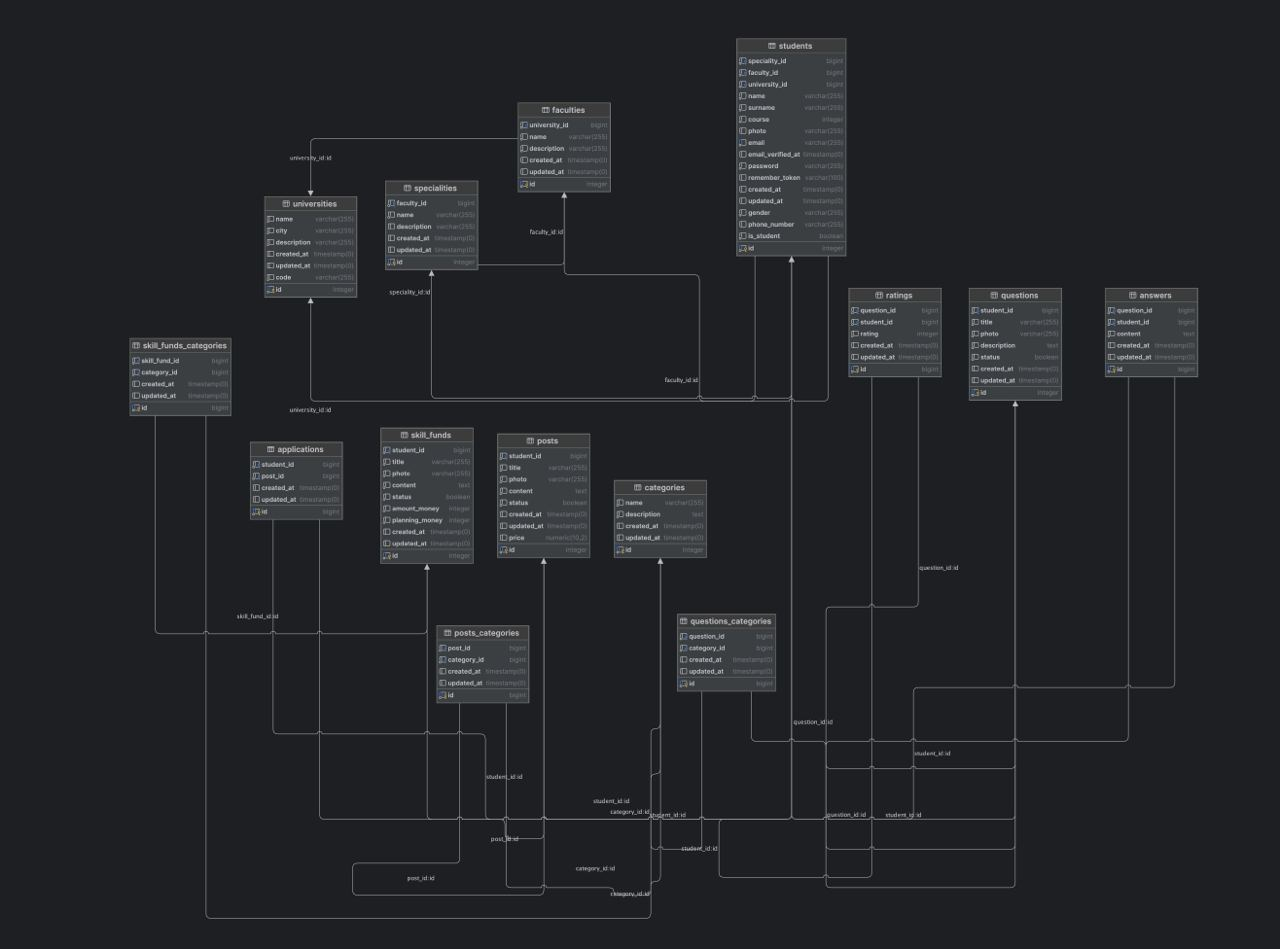
\includegraphics[width=0.8\linewidth]{figures/Database.jpg}
  \caption{Database.}
\end{figure}
\section{Jira Backlog}\label{backlog}
\begin{figure}[H]\label{fig:jira}
  \centering
  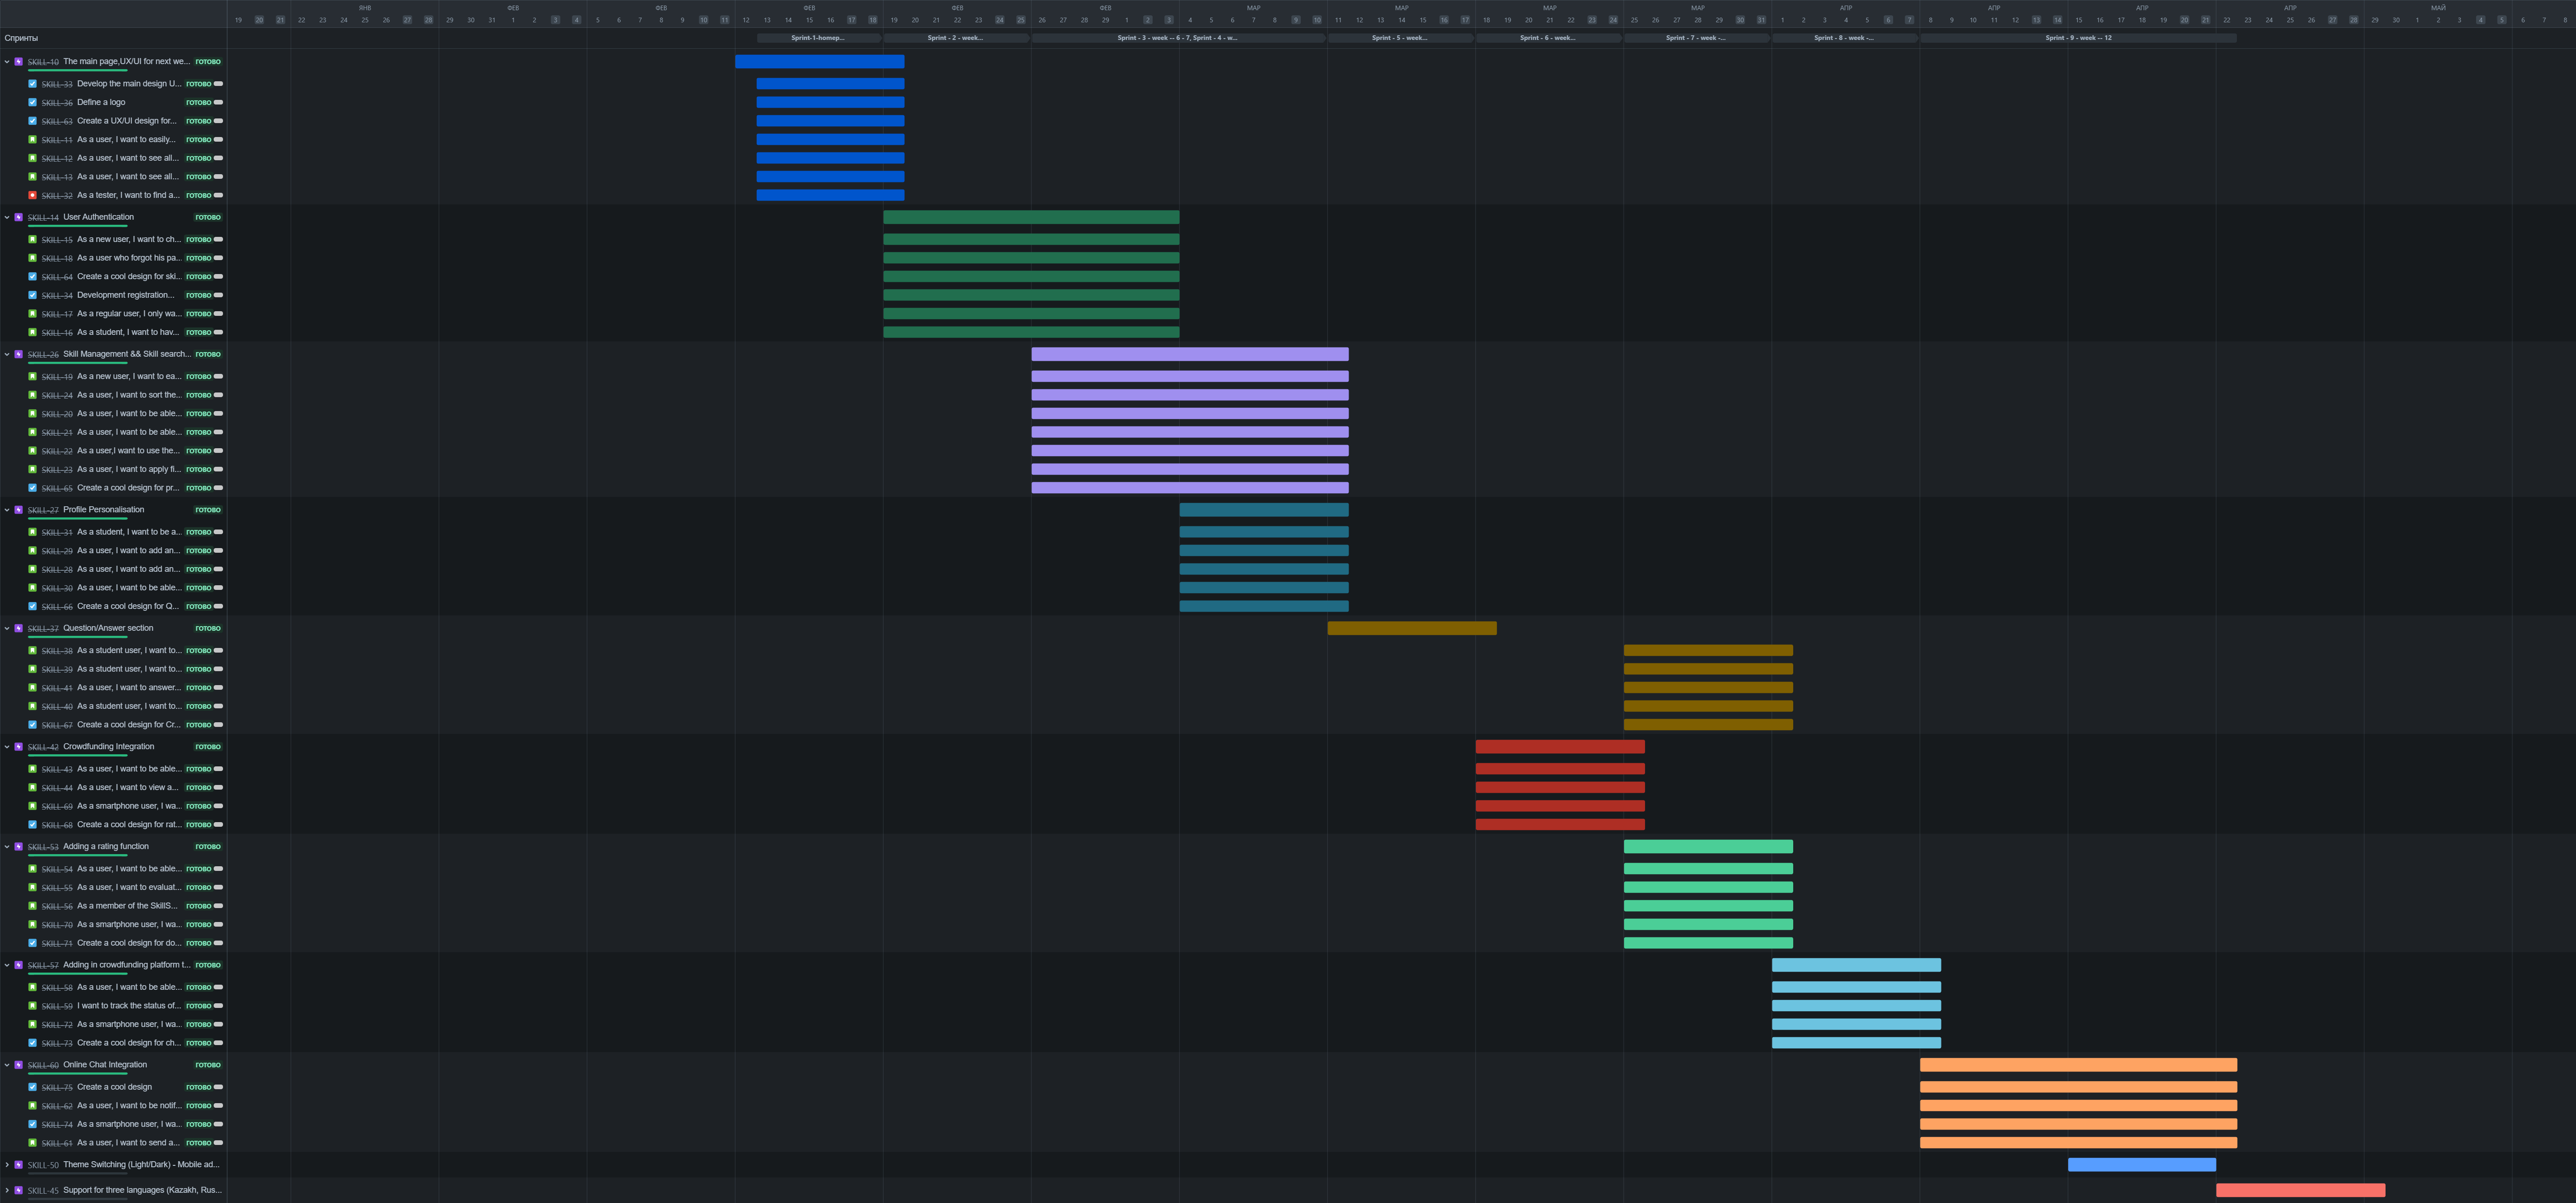
\includegraphics[width=0.8\linewidth]{figures/skill_swap_development____crowd_funding_platform_2024-04-28_03.06pm.png}
  \caption{Jira backlog.}
\end{figure}
\section{Telegram Channel}\label{telegram}
\begin{figure}[H]\label{fig:telegram}
  \centering
  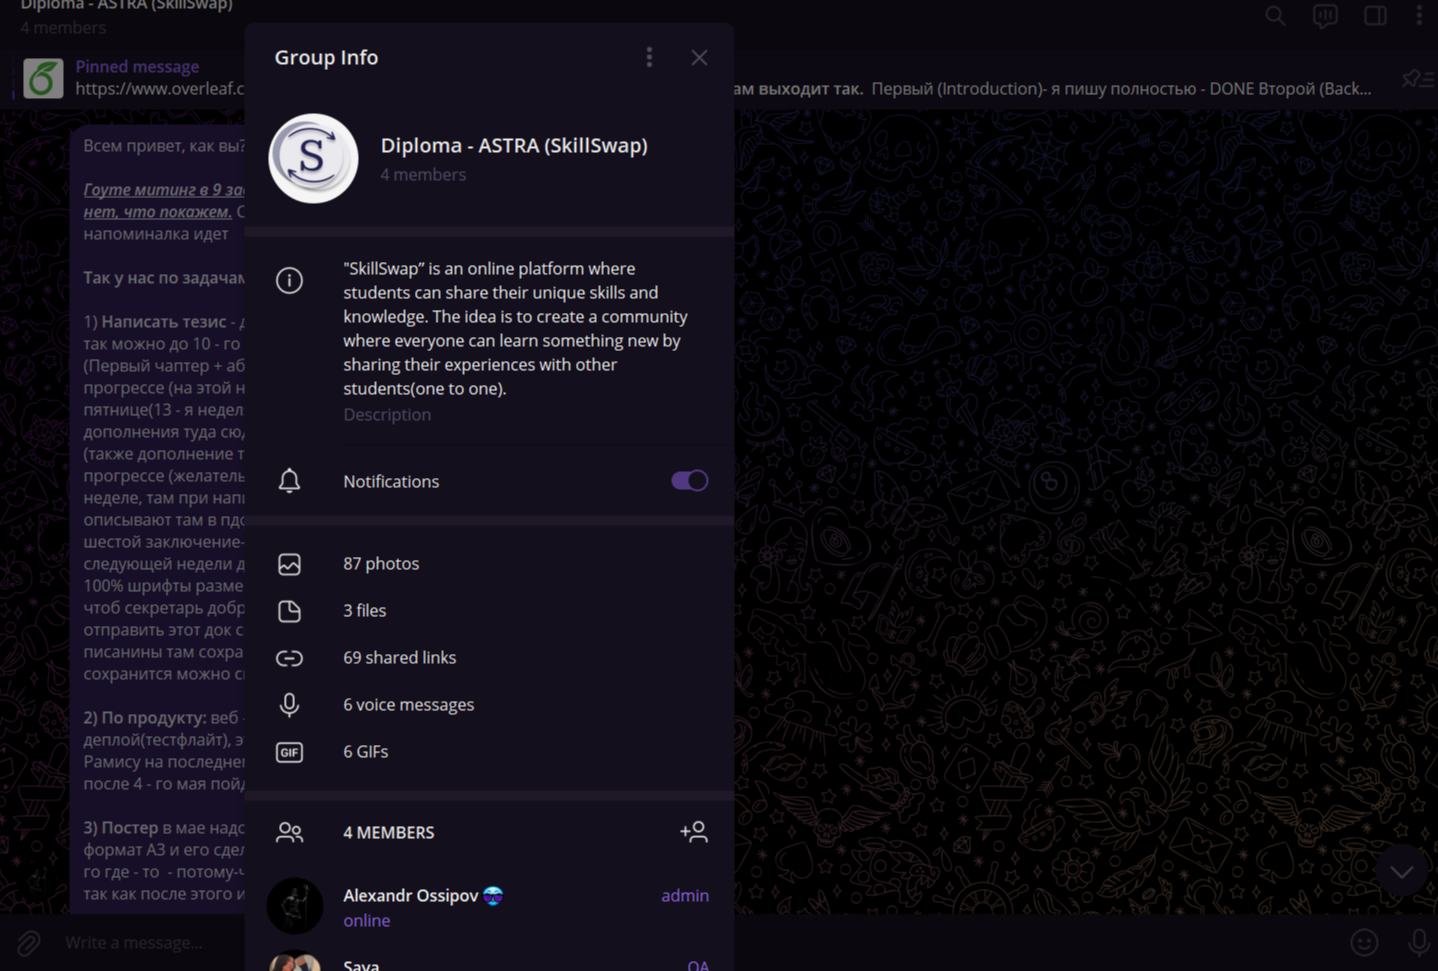
\includegraphics[width=0.8\linewidth]{figures/Telegram group.png}
  \caption{Telegram group.}
\end{figure}
\section{Daily Stand-up}\label{standup}
\begin{figure}[H]\label{fig:standup}
  \centering
  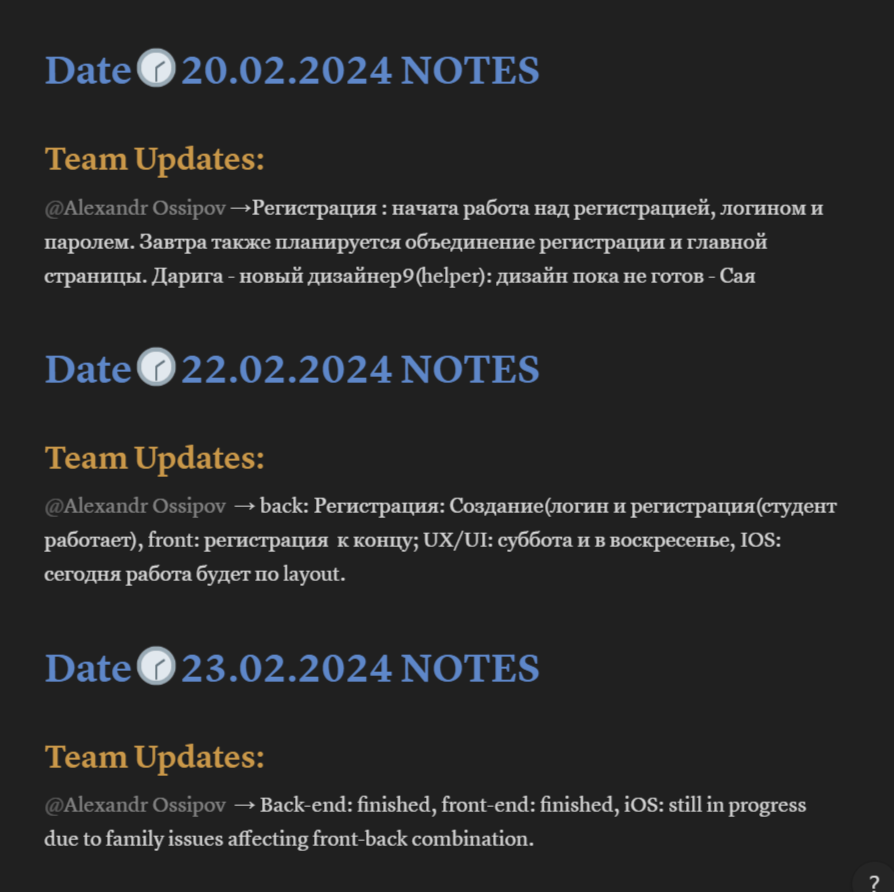
\includegraphics[width=0.8\linewidth]{figures/Daily standup.png}
  \caption{Daily stand-up.}
\end{figure}
\section{Survey Question 1}\label{survqa1}
\begin{figure}[H]\label{fig:survey1}
  \centering
  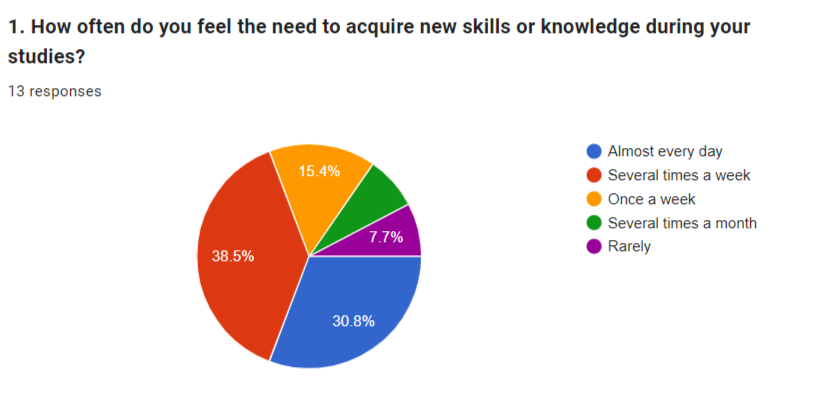
\includegraphics[width=0.8\linewidth]{figures/Survey question 1.png}
  \caption{Survey 1.}
\end{figure}
\section{Survey Question 2}\label{survqa2}
\begin{figure}[H]\label{fig:survey2}
  \centering
  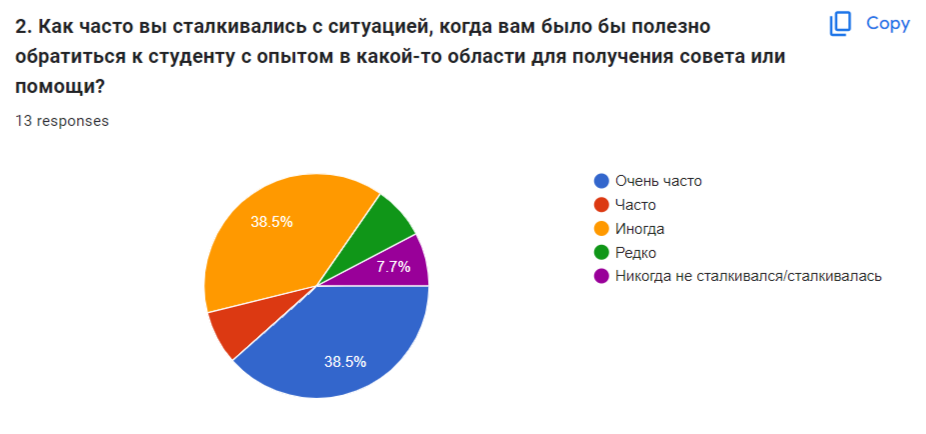
\includegraphics[width=0.8\linewidth]{figures/Survey question 2.png}
  \caption{Survey 2.}
\end{figure}
\section{Survey Question 3}\label{survqa3}
\begin{figure}[H]\label{fig:survey3}
  \centering
  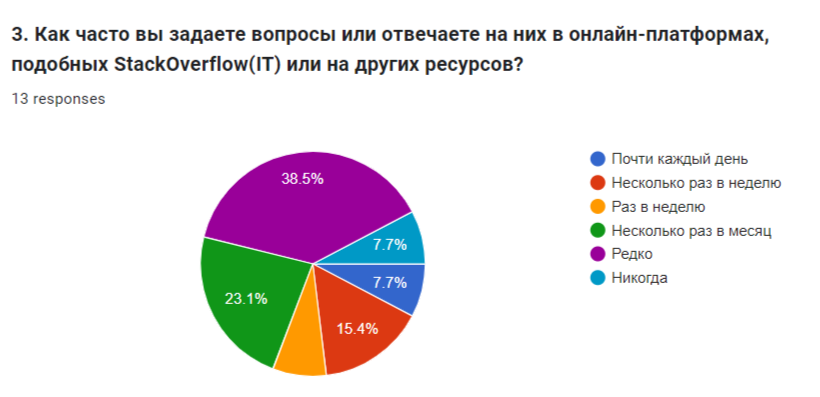
\includegraphics[width=0.8\linewidth]{figures/Survey question 3.png}
  \caption{Survey 3.}
\end{figure}
\section{Survey Question 4}\label{survqa4}
\begin{figure}[H]\label{fig:survey4}
  \centering
  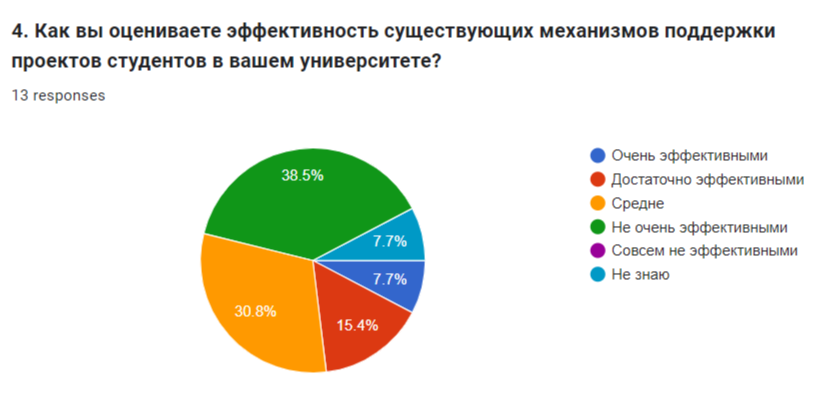
\includegraphics[width=0.8\linewidth]{figures/Survey question 4.png}
  \caption{Survey 4.}
\end{figure}
\section{Survey Question 5}\label{survqa5}
\begin{figure}[H]\label{fig:survey5}
  \centering
  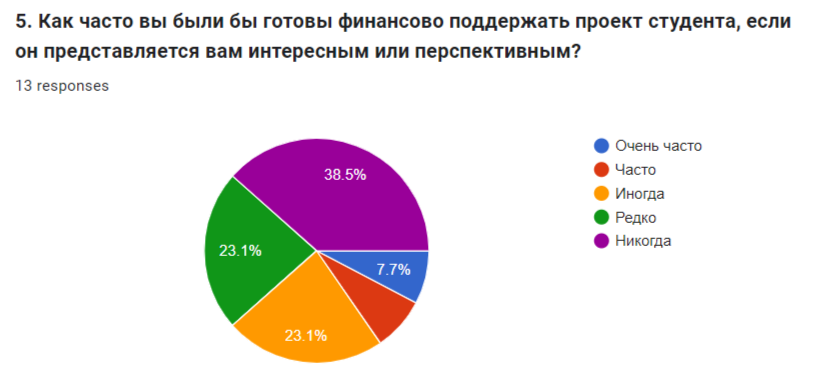
\includegraphics[width=0.8\linewidth]{figures/Survey question 5.png}
  \caption{Survey 5.}
\end{figure}
\section{Survey Question 6}\label{survqa6}
\begin{figure}[H]\label{fig:survey6}
  \centering
  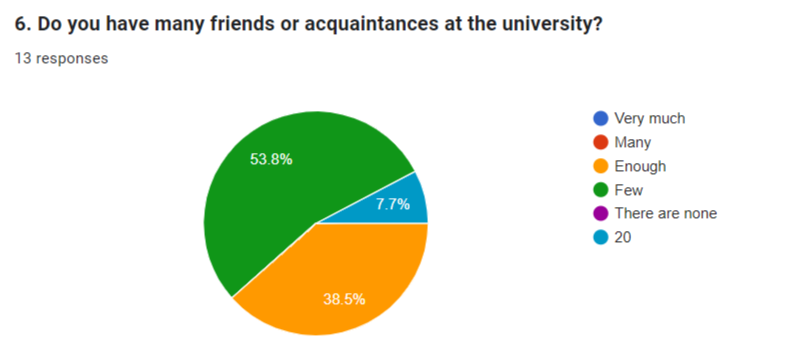
\includegraphics[width=0.8\linewidth]{figures/Survey question 6.png}
  \caption{Survey 6.}
\end{figure}
\section{Low Fidelity Design}\label{lowdesign}
\begin{figure}[H]\label{fig:lowdesign}
  \centering
  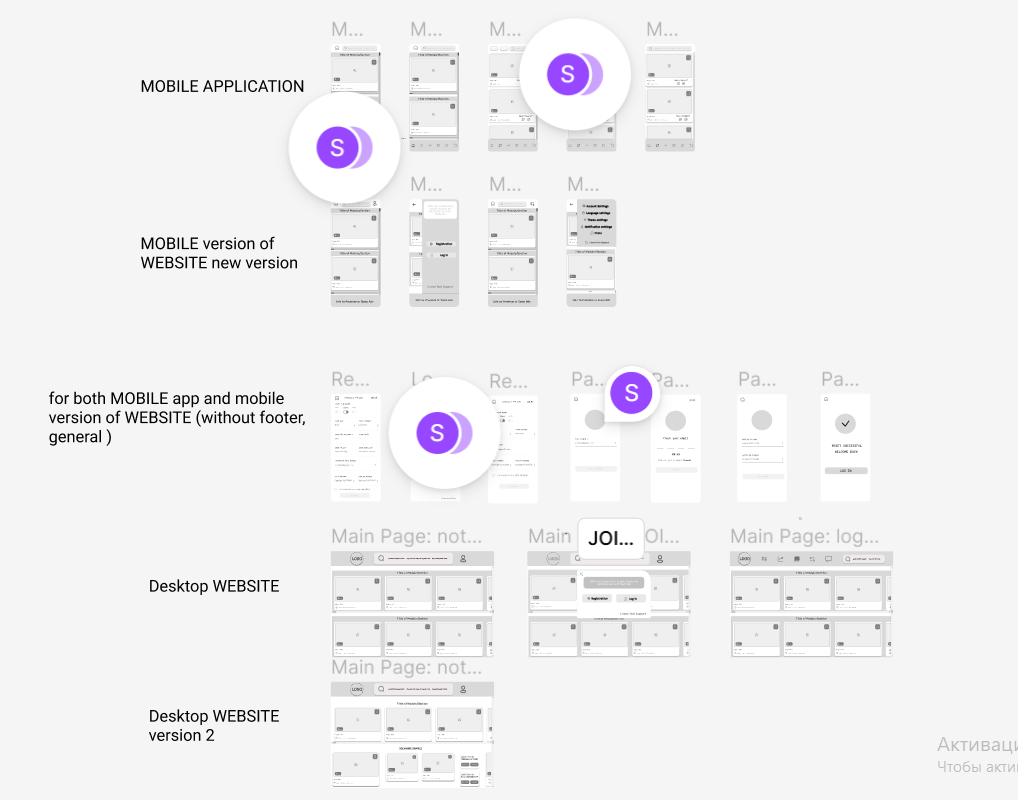
\includegraphics[width=0.8\linewidth]{figures/wireframe.png}
  \caption{Low design.}
\end{figure}
    \chapter{Chapter B}\label{app:BB}
\section{PhP URLs code}
\begin{lstlisting}[style=php, caption={PHP URLs code}]
<?php

// Create Post
URL:/posts/create
Method:{POST}
Description: Allows a student to create a new post.
Request Body: JSON containing post details.
Authorization: Requires a valid authentication token.

// Apply for Post
URL:/posts/\{post\}/apply
Method:{POST}
Description: Allows a student to apply for a specific post.
URL Parameters: ID of the post.
Authorization: Requires a valid authentication token.

// Update Post
URL:/posts/\{id\}/update
Method:{PUT}
Description: Allows updating an existing post.
URL Parameters: ID of the post.
Request Body: JSON containing updated post details.
Authorization: Requires a valid authentication token.

// Delete Post
URL:/posts/\{post\}/delete
Method:{DELETE}
Description: Allows deleting an existing post.
URL Parameters: ID of the post.
Authorization: Requires a valid authentication token.

// Search Questions
URL:/questions/search
Method:{GET}
Description: Allows searching for questions based on criteria.
Query Parameters: Keywords for search.
Authorization: Requires a valid authentication token.

// Retrieve All Questions
URL:questions/all
Method:{GET}
Description: Retrieves all questions in the system.
Authorization: Requires a valid authentication token.

// Create Question
URL:/questions/create
Method:{POST}
Description: Allows a student to create a new question.
Request Body: JSON containing question details.
Authorization: Requires a valid authentication token.

// Rate Question
URL:/questions/\{id\}/rate
Method:{POST}
Description: Allows a student to rate a specific question.
URL Parameters: ID of the question.
Request Body: JSON containing rating details (+1 for like, -1 for dislike).
Authorization: Requires a valid authentication token.

// Update Question
URL:/questions/\{id\}/update
Method:{PUT}
Description: Allows updating an existing question.
URL Parameters: ID of the question.
Request Body: JSON containing updated question details.
Authorization: Requires a valid authentication token.

// Delete Question
URL:/questions/\{id\}/delete
Method:{DELETE}
Description: Allows deleting an existing question.
URL Parameters: ID of the question.
Authorization: Requires a valid authentication token.

// Retrieve Profile
URL:/student/profile
Method:{GET}
Description: Retrieves the profile of the authenticated student.
Authorization: Requires a valid authentication token.

// Update Profile
URL:/student/profile/update
Method:{PUT}
Description: Allows updating the profile of the authenticated student.
Request Body JSON containing updated profile details.
Authorization: Requires a valid authentication token.
\end{lstlisting}

\section{Pagination in Back - end}
\begin{figure}[H]\label{fig:pagination}
  \centering
  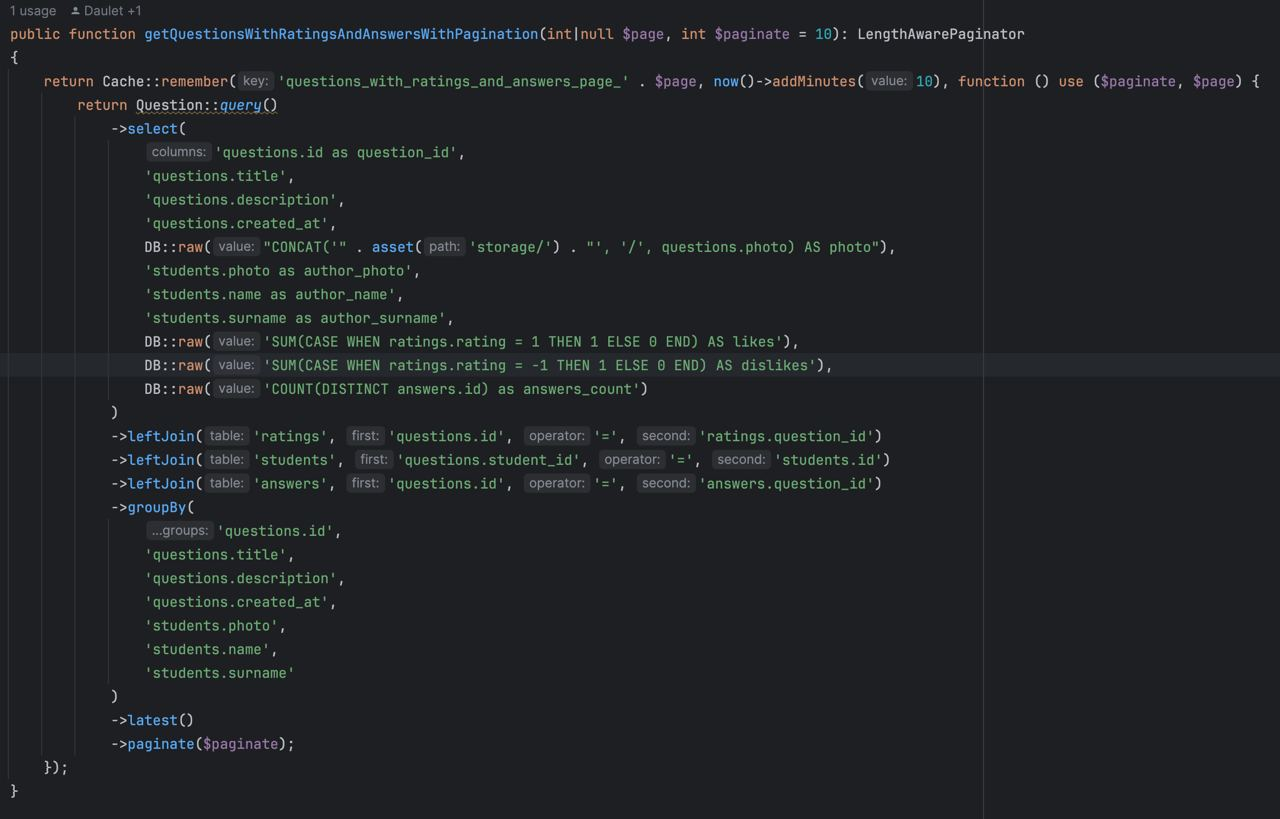
\includegraphics[width=0.8\linewidth]{figures/Pagination.jpg}
  \caption{Pagination.}
\end{figure}
\section{IOS Screens of codes}
\begin{figure}[H]\label{fig:authorization}
  \centering
  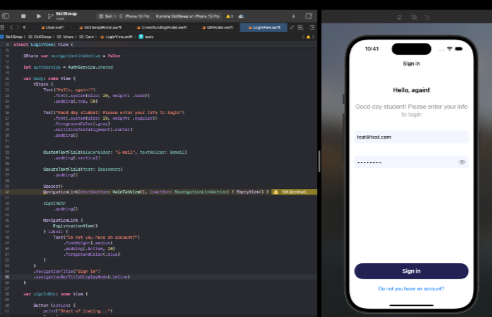
\includegraphics[width=0.8\linewidth]{figures/Authorization.png}
  \caption{Authorization.}
\end{figure}
\begin{figure}[H]\label{fig:skillsharingmodel}
  \centering
  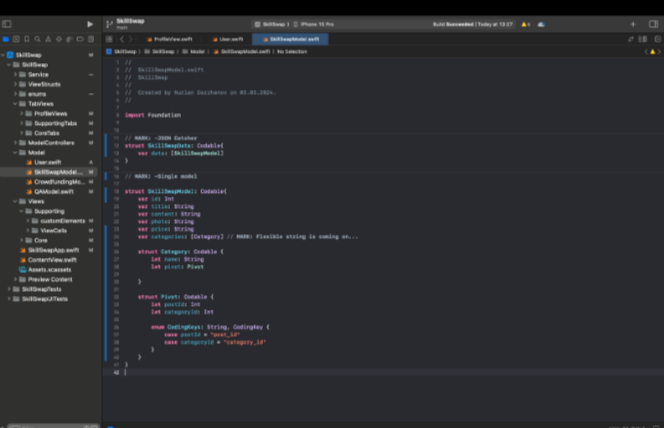
\includegraphics[width=0.8\linewidth]{figures/Skill Sharing model.png}
  \caption{Skill Sharing model.}
\end{figure}
\begin{figure}[H]\label{fig:crowdfundingmodel}
  \centering
  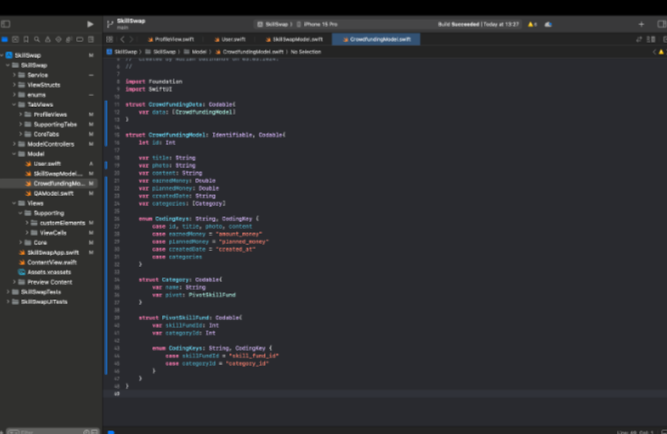
\includegraphics[width=0.8\linewidth]{figures/Crowdfunding model.png}
  \caption{Crowdfunding model.}
\end{figure}
\begin{figure}[H]\label{fig:questionanswerModel}
  \centering
  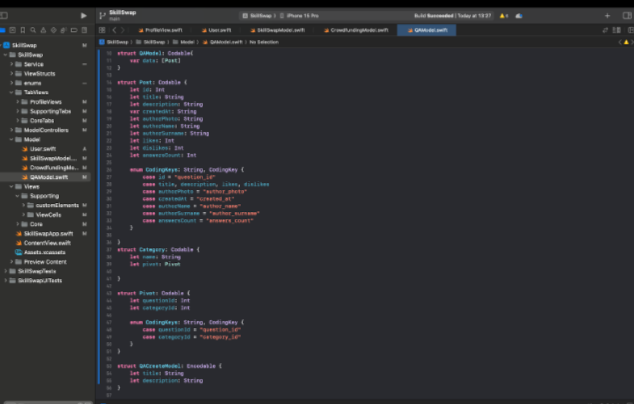
\includegraphics[width=0.8\linewidth]{figures/Question and Answer (QA) Model.png}
  \caption{Question and Answer (QA) Model.}
\end{figure}
\begin{figure}[H]\label{fig:registration}
  \centering
  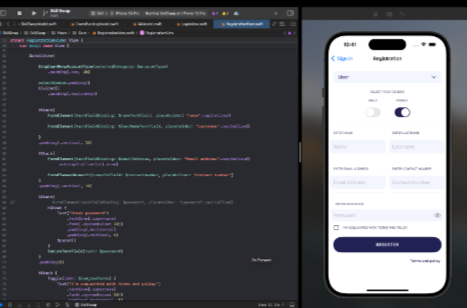
\includegraphics[width=0.8\linewidth]{figures/Registration.png}
  \caption{Registration.}
\end{figure}
\begin{figure}[H]\label{fig:authorizationmodel}
  \centering
  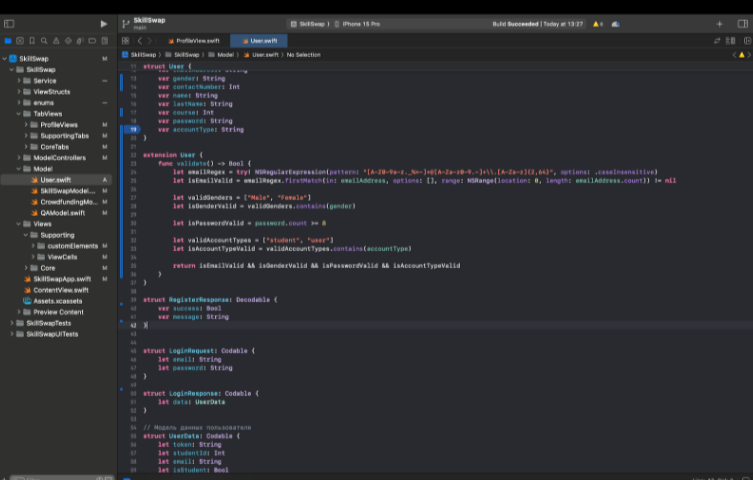
\includegraphics[width=0.8\linewidth]{figures/Authorization model.png}
  \caption{Authorization model.}
\end{figure}
\begin{figure}[H]\label{fig:createpstskillswap}
  \centering
  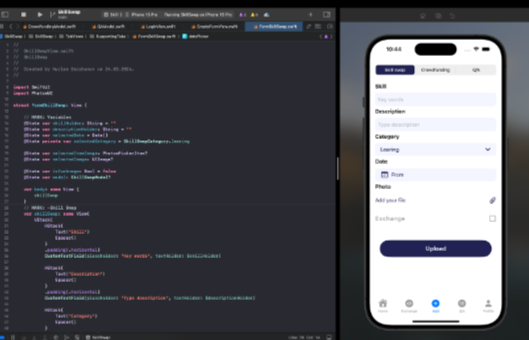
\includegraphics[width=0.8\linewidth]{figures/Creating a post (Skill Swap).png}
  \caption{Creating a post (Skill Swap).}
\end{figure}
\begin{figure}[H]\label{fig:createpstcrowd}
  \centering
  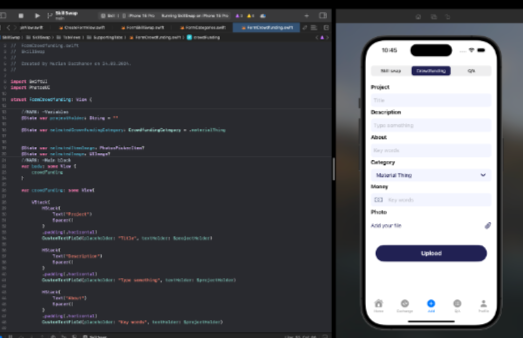
\includegraphics[width=0.8\linewidth]{figures/Create a post (Crowdfund).png}
  \caption{Create a post (Crowdfund).}
\end{figure}
\begin{figure}[H]\label{fig:createpstq}
  \centering
  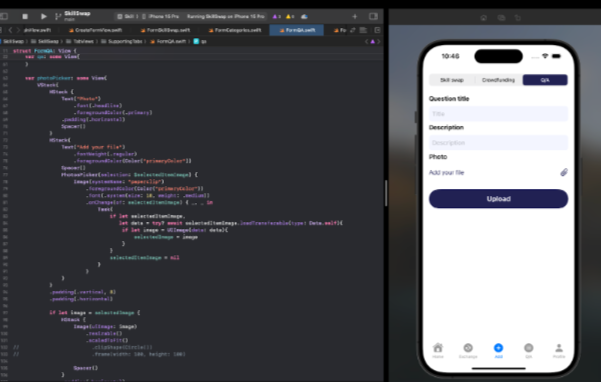
\includegraphics[width=0.8\linewidth]{figures/Crate a post (Question).png}
  \caption{Crate a post (Question).}
\end{figure}
    
\justifying
\printbibliography[heading=bibintoc,title={References}]
\end{document}
